% Options for packages loaded elsewhere
\PassOptionsToPackage{unicode}{hyperref}
\PassOptionsToPackage{hyphens}{url}
%
\documentclass[
]{article}
\usepackage{amsmath,amssymb}
\usepackage{iftex}
\ifPDFTeX
  \usepackage[T1]{fontenc}
  \usepackage[utf8]{inputenc}
  \usepackage{textcomp} % provide euro and other symbols
\else % if luatex or xetex
  \usepackage{unicode-math} % this also loads fontspec
  \defaultfontfeatures{Scale=MatchLowercase}
  \defaultfontfeatures[\rmfamily]{Ligatures=TeX,Scale=1}
\fi
\usepackage{lmodern}
\ifPDFTeX\else
  % xetex/luatex font selection
\fi
% Use upquote if available, for straight quotes in verbatim environments
\IfFileExists{upquote.sty}{\usepackage{upquote}}{}
\IfFileExists{microtype.sty}{% use microtype if available
  \usepackage[]{microtype}
  \UseMicrotypeSet[protrusion]{basicmath} % disable protrusion for tt fonts
}{}
\makeatletter
\@ifundefined{KOMAClassName}{% if non-KOMA class
  \IfFileExists{parskip.sty}{%
    \usepackage{parskip}
  }{% else
    \setlength{\parindent}{0pt}
    \setlength{\parskip}{6pt plus 2pt minus 1pt}}
}{% if KOMA class
  \KOMAoptions{parskip=half}}
\makeatother
\usepackage{xcolor}
\usepackage[margin=1in]{geometry}
\usepackage{color}
\usepackage{fancyvrb}
\newcommand{\VerbBar}{|}
\newcommand{\VERB}{\Verb[commandchars=\\\{\}]}
\DefineVerbatimEnvironment{Highlighting}{Verbatim}{commandchars=\\\{\}}
% Add ',fontsize=\small' for more characters per line
\usepackage{framed}
\definecolor{shadecolor}{RGB}{248,248,248}
\newenvironment{Shaded}{\begin{snugshade}}{\end{snugshade}}
\newcommand{\AlertTok}[1]{\textcolor[rgb]{0.94,0.16,0.16}{#1}}
\newcommand{\AnnotationTok}[1]{\textcolor[rgb]{0.56,0.35,0.01}{\textbf{\textit{#1}}}}
\newcommand{\AttributeTok}[1]{\textcolor[rgb]{0.13,0.29,0.53}{#1}}
\newcommand{\BaseNTok}[1]{\textcolor[rgb]{0.00,0.00,0.81}{#1}}
\newcommand{\BuiltInTok}[1]{#1}
\newcommand{\CharTok}[1]{\textcolor[rgb]{0.31,0.60,0.02}{#1}}
\newcommand{\CommentTok}[1]{\textcolor[rgb]{0.56,0.35,0.01}{\textit{#1}}}
\newcommand{\CommentVarTok}[1]{\textcolor[rgb]{0.56,0.35,0.01}{\textbf{\textit{#1}}}}
\newcommand{\ConstantTok}[1]{\textcolor[rgb]{0.56,0.35,0.01}{#1}}
\newcommand{\ControlFlowTok}[1]{\textcolor[rgb]{0.13,0.29,0.53}{\textbf{#1}}}
\newcommand{\DataTypeTok}[1]{\textcolor[rgb]{0.13,0.29,0.53}{#1}}
\newcommand{\DecValTok}[1]{\textcolor[rgb]{0.00,0.00,0.81}{#1}}
\newcommand{\DocumentationTok}[1]{\textcolor[rgb]{0.56,0.35,0.01}{\textbf{\textit{#1}}}}
\newcommand{\ErrorTok}[1]{\textcolor[rgb]{0.64,0.00,0.00}{\textbf{#1}}}
\newcommand{\ExtensionTok}[1]{#1}
\newcommand{\FloatTok}[1]{\textcolor[rgb]{0.00,0.00,0.81}{#1}}
\newcommand{\FunctionTok}[1]{\textcolor[rgb]{0.13,0.29,0.53}{\textbf{#1}}}
\newcommand{\ImportTok}[1]{#1}
\newcommand{\InformationTok}[1]{\textcolor[rgb]{0.56,0.35,0.01}{\textbf{\textit{#1}}}}
\newcommand{\KeywordTok}[1]{\textcolor[rgb]{0.13,0.29,0.53}{\textbf{#1}}}
\newcommand{\NormalTok}[1]{#1}
\newcommand{\OperatorTok}[1]{\textcolor[rgb]{0.81,0.36,0.00}{\textbf{#1}}}
\newcommand{\OtherTok}[1]{\textcolor[rgb]{0.56,0.35,0.01}{#1}}
\newcommand{\PreprocessorTok}[1]{\textcolor[rgb]{0.56,0.35,0.01}{\textit{#1}}}
\newcommand{\RegionMarkerTok}[1]{#1}
\newcommand{\SpecialCharTok}[1]{\textcolor[rgb]{0.81,0.36,0.00}{\textbf{#1}}}
\newcommand{\SpecialStringTok}[1]{\textcolor[rgb]{0.31,0.60,0.02}{#1}}
\newcommand{\StringTok}[1]{\textcolor[rgb]{0.31,0.60,0.02}{#1}}
\newcommand{\VariableTok}[1]{\textcolor[rgb]{0.00,0.00,0.00}{#1}}
\newcommand{\VerbatimStringTok}[1]{\textcolor[rgb]{0.31,0.60,0.02}{#1}}
\newcommand{\WarningTok}[1]{\textcolor[rgb]{0.56,0.35,0.01}{\textbf{\textit{#1}}}}
\usepackage{longtable,booktabs,array}
\usepackage{calc} % for calculating minipage widths
% Correct order of tables after \paragraph or \subparagraph
\usepackage{etoolbox}
\makeatletter
\patchcmd\longtable{\par}{\if@noskipsec\mbox{}\fi\par}{}{}
\makeatother
% Allow footnotes in longtable head/foot
\IfFileExists{footnotehyper.sty}{\usepackage{footnotehyper}}{\usepackage{footnote}}
\makesavenoteenv{longtable}
\usepackage{graphicx}
\makeatletter
\def\maxwidth{\ifdim\Gin@nat@width>\linewidth\linewidth\else\Gin@nat@width\fi}
\def\maxheight{\ifdim\Gin@nat@height>\textheight\textheight\else\Gin@nat@height\fi}
\makeatother
% Scale images if necessary, so that they will not overflow the page
% margins by default, and it is still possible to overwrite the defaults
% using explicit options in \includegraphics[width, height, ...]{}
\setkeys{Gin}{width=\maxwidth,height=\maxheight,keepaspectratio}
% Set default figure placement to htbp
\makeatletter
\def\fps@figure{htbp}
\makeatother
\setlength{\emergencystretch}{3em} % prevent overfull lines
\providecommand{\tightlist}{%
  \setlength{\itemsep}{0pt}\setlength{\parskip}{0pt}}
\setcounter{secnumdepth}{5}
% definitions for citeproc citations
\NewDocumentCommand\citeproctext{}{}
\NewDocumentCommand\citeproc{mm}{%
  \begingroup\def\citeproctext{#2}\cite{#1}\endgroup}
\makeatletter
 % allow citations to break across lines
 \let\@cite@ofmt\@firstofone
 % avoid brackets around text for \cite:
 \def\@biblabel#1{}
 \def\@cite#1#2{{#1\if@tempswa , #2\fi}}
\makeatother
\newlength{\cslhangindent}
\setlength{\cslhangindent}{1.5em}
\newlength{\csllabelwidth}
\setlength{\csllabelwidth}{3em}
\newenvironment{CSLReferences}[2] % #1 hanging-indent, #2 entry-spacing
 {\begin{list}{}{%
  \setlength{\itemindent}{0pt}
  \setlength{\leftmargin}{0pt}
  \setlength{\parsep}{0pt}
  % turn on hanging indent if param 1 is 1
  \ifodd #1
   \setlength{\leftmargin}{\cslhangindent}
   \setlength{\itemindent}{-1\cslhangindent}
  \fi
  % set entry spacing
  \setlength{\itemsep}{#2\baselineskip}}}
 {\end{list}}
\usepackage{calc}
\newcommand{\CSLBlock}[1]{\hfill\break\parbox[t]{\linewidth}{\strut\ignorespaces#1\strut}}
\newcommand{\CSLLeftMargin}[1]{\parbox[t]{\csllabelwidth}{\strut#1\strut}}
\newcommand{\CSLRightInline}[1]{\parbox[t]{\linewidth - \csllabelwidth}{\strut#1\strut}}
\newcommand{\CSLIndent}[1]{\hspace{\cslhangindent}#1}
\usepackage{graphicx}
\usepackage{titling}

\pretitle{}
\posttitle{}

\preauthor{}
\postauthor{}

\predate{}
\postdate{}

\renewcommand{\maketitle}{
  \begin{center}
    \vspace*{2cm}
    {\Huge \textbf{Part A, Topic 2 - Olympic Tweets}}\\[1.5cm]  % Title
    
\includegraphics[width=0.3\textwidth]{Monash University.png}\\[1.5cm]  % Logo (logo.png must be in the same folder)
    {\LARGE \textbf{Lance Belen}}\\[1.5cm]  % Author
    \vspace*{1cm}
    \today
    \vfill
  \end{center}
  \newpage
}
\ifLuaTeX
  \usepackage{selnolig}  % disable illegal ligatures
\fi
\usepackage{bookmark}
\IfFileExists{xurl.sty}{\usepackage{xurl}}{} % add URL line breaks if available
\urlstyle{same}
\hypersetup{
  pdftitle={Part A, Topic 2 - Olympic Tweets},
  pdfauthor={Lance Belen},
  hidelinks,
  pdfcreator={LaTeX via pandoc}}

\title{Part A, Topic 2 - Olympic Tweets}
\author{Lance Belen}
\date{2 June 2025}

\begin{document}
\maketitle

{
\setcounter{tocdepth}{2}
\tableofcontents
}
\newpage

\section{Data Wrangling, Visualisatsion, and
Analysis}\label{data-wrangling-visualisatsion-and-analysis}

First, load the packages needed.

\begin{Shaded}
\begin{Highlighting}[]
\FunctionTok{options}\NormalTok{(}\AttributeTok{repos =} \FunctionTok{c}\NormalTok{(}\AttributeTok{CRAN =} \StringTok{"https://cloud.r{-}project.org/"}\NormalTok{))}

\ControlFlowTok{if}\NormalTok{ (}\SpecialCharTok{!}\FunctionTok{requireNamespace}\NormalTok{(}\StringTok{"tidyverse"}\NormalTok{, }\AttributeTok{quietly =} \ConstantTok{TRUE}\NormalTok{)) \{}
  \FunctionTok{install.packages}\NormalTok{(}\StringTok{"tidyverse"}\NormalTok{)}
\NormalTok{\}}
\ControlFlowTok{if}\NormalTok{ (}\SpecialCharTok{!}\FunctionTok{requireNamespace}\NormalTok{(}\StringTok{"lubridate"}\NormalTok{, }\AttributeTok{quietly =} \ConstantTok{TRUE}\NormalTok{)) \{}
  \FunctionTok{install.packages}\NormalTok{(}\StringTok{"lubridate"}\NormalTok{)}
\NormalTok{\}}
\ControlFlowTok{if}\NormalTok{ (}\SpecialCharTok{!}\FunctionTok{requireNamespace}\NormalTok{(}\StringTok{"impute"}\NormalTok{, }\AttributeTok{quietly =} \ConstantTok{TRUE}\NormalTok{)) \{}
  \FunctionTok{install.packages}\NormalTok{(}\StringTok{"impute"}\NormalTok{)}
\NormalTok{\}}
\ControlFlowTok{if}\NormalTok{ (}\SpecialCharTok{!}\FunctionTok{requireNamespace}\NormalTok{(}\StringTok{"dplyr"}\NormalTok{, }\AttributeTok{quietly =} \ConstantTok{TRUE}\NormalTok{)) \{}
  \FunctionTok{install.packages}\NormalTok{(}\StringTok{"dplyr"}\NormalTok{)}
\NormalTok{\}}
\ControlFlowTok{if}\NormalTok{ (}\SpecialCharTok{!}\FunctionTok{requireNamespace}\NormalTok{(}\StringTok{"magrittr"}\NormalTok{, }\AttributeTok{quietly =} \ConstantTok{TRUE}\NormalTok{)) \{}
  \FunctionTok{install.packages}\NormalTok{(}\StringTok{"magrittr"}\NormalTok{)}
\NormalTok{\}}
\ControlFlowTok{if}\NormalTok{ (}\SpecialCharTok{!}\FunctionTok{requireNamespace}\NormalTok{(}\StringTok{"ggplot2"}\NormalTok{, }\AttributeTok{quietly =} \ConstantTok{TRUE}\NormalTok{)) \{}
  \FunctionTok{install.packages}\NormalTok{(}\StringTok{"ggplot2"}\NormalTok{)}
\NormalTok{\}}
\ControlFlowTok{if}\NormalTok{ (}\SpecialCharTok{!}\FunctionTok{requireNamespace}\NormalTok{(}\StringTok{"readxl"}\NormalTok{, }\AttributeTok{quietly =} \ConstantTok{TRUE}\NormalTok{)) \{}
  \FunctionTok{install.packages}\NormalTok{(}\StringTok{"readxl"}\NormalTok{)}
\NormalTok{\}}
\ControlFlowTok{if}\NormalTok{ (}\SpecialCharTok{!}\FunctionTok{requireNamespace}\NormalTok{(}\StringTok{"stringr"}\NormalTok{, }\AttributeTok{quietly =} \ConstantTok{TRUE}\NormalTok{)) \{}
  \FunctionTok{install.packages}\NormalTok{(}\StringTok{"stringr"}\NormalTok{)}
\NormalTok{\}}
\ControlFlowTok{if}\NormalTok{ (}\SpecialCharTok{!}\FunctionTok{requireNamespace}\NormalTok{(}\StringTok{"forcats"}\NormalTok{, }\AttributeTok{quietly =} \ConstantTok{TRUE}\NormalTok{)) \{}
  \FunctionTok{install.packages}\NormalTok{(}\StringTok{"forcats"}\NormalTok{)}
\NormalTok{\}}
\ControlFlowTok{if}\NormalTok{ (}\SpecialCharTok{!}\FunctionTok{requireNamespace}\NormalTok{(}\StringTok{"tidytext"}\NormalTok{, }\AttributeTok{quietly =} \ConstantTok{TRUE}\NormalTok{)) \{}
  \FunctionTok{install.packages}\NormalTok{(}\StringTok{"tidytext"}\NormalTok{)}
\NormalTok{\}}
\ControlFlowTok{if}\NormalTok{(}\SpecialCharTok{!}\FunctionTok{requireNamespace}\NormalTok{(}\StringTok{"xgboost"}\NormalTok{, }\AttributeTok{quietly =} \ConstantTok{TRUE}\NormalTok{)) \{}
  \FunctionTok{install.packages}\NormalTok{(}\StringTok{"xgboost"}\NormalTok{)}
\NormalTok{\}}
\ControlFlowTok{if}\NormalTok{(}\SpecialCharTok{!}\FunctionTok{requireNamespace}\NormalTok{(}\StringTok{"MLmetrics"}\NormalTok{, }\AttributeTok{quietly =} \ConstantTok{TRUE}\NormalTok{)) \{}
  \FunctionTok{install.packages}\NormalTok{(}\StringTok{"MLmetrics"}\NormalTok{)}
\NormalTok{\}}

\FunctionTok{library}\NormalTok{(tidyverse)}
\FunctionTok{library}\NormalTok{(lubridate)}
\FunctionTok{library}\NormalTok{(impute)}
\FunctionTok{library}\NormalTok{(dplyr)}
\FunctionTok{library}\NormalTok{(magrittr)}
\FunctionTok{library}\NormalTok{(ggplot2)}
\FunctionTok{library}\NormalTok{(readxl)}
\FunctionTok{library}\NormalTok{(stringr)}
\FunctionTok{library}\NormalTok{(forcats)}
\FunctionTok{library}\NormalTok{(tidytext)}
\FunctionTok{library}\NormalTok{(xgboost)}
\FunctionTok{library}\NormalTok{(MLmetrics)}
\end{Highlighting}
\end{Shaded}

\subsection{Data Wrangling}\label{data-wrangling}

Then, read and open the dataset.

\begin{Shaded}
\begin{Highlighting}[]
\NormalTok{tweets }\OtherTok{\textless{}{-}} \FunctionTok{read.csv}\NormalTok{(}\StringTok{"Olympics\_tweets.csv"}\NormalTok{)}
\end{Highlighting}
\end{Shaded}

Next, explore the dataset.

\begin{Shaded}
\begin{Highlighting}[]
\FunctionTok{cat}\NormalTok{(}\StringTok{"Number of rows: "}\NormalTok{, }\FunctionTok{nrow}\NormalTok{(tweets), }\StringTok{"}\SpecialCharTok{\textbackslash{}n}\StringTok{"}\NormalTok{)}
\FunctionTok{cat}\NormalTok{(}\StringTok{"Number of columns: "}\NormalTok{, }\FunctionTok{ncol}\NormalTok{(tweets), }\StringTok{"}\SpecialCharTok{\textbackslash{}n}\StringTok{"}\NormalTok{)}
\NormalTok{knitr}\SpecialCharTok{::}\FunctionTok{kable}\NormalTok{(}\FunctionTok{head}\NormalTok{(tweets))}
\FunctionTok{cat}\NormalTok{(}\StringTok{"Structure of the dataset: }\SpecialCharTok{\textbackslash{}n}\StringTok{"}\NormalTok{)}
\FunctionTok{str}\NormalTok{(tweets)}
\FunctionTok{cat}\NormalTok{(}\StringTok{"Summary of the dataset: }\SpecialCharTok{\textbackslash{}n}\StringTok{"}\NormalTok{)}
\FunctionTok{summary}\NormalTok{(tweets)}
\end{Highlighting}
\end{Shaded}

\begin{verbatim}
## Number of rows:  114213
\end{verbatim}

\begin{verbatim}
## Number of columns:  13
\end{verbatim}

\begin{longtable}[]{@{}
  >{\raggedleft\arraybackslash}p{(\columnwidth - 24\tabcolsep) * \real{0.0278}}
  >{\raggedright\arraybackslash}p{(\columnwidth - 24\tabcolsep) * \real{0.3098}}
  >{\raggedright\arraybackslash}p{(\columnwidth - 24\tabcolsep) * \real{0.0363}}
  >{\raggedright\arraybackslash}p{(\columnwidth - 24\tabcolsep) * \real{0.0491}}
  >{\raggedleft\arraybackslash}p{(\columnwidth - 24\tabcolsep) * \real{0.0299}}
  >{\raggedright\arraybackslash}p{(\columnwidth - 24\tabcolsep) * \real{0.0214}}
  >{\raggedleft\arraybackslash}p{(\columnwidth - 24\tabcolsep) * \real{0.0321}}
  >{\raggedright\arraybackslash}p{(\columnwidth - 24\tabcolsep) * \real{0.3419}}
  >{\raggedright\arraybackslash}p{(\columnwidth - 24\tabcolsep) * \real{0.0363}}
  >{\raggedleft\arraybackslash}p{(\columnwidth - 24\tabcolsep) * \real{0.0321}}
  >{\raggedleft\arraybackslash}p{(\columnwidth - 24\tabcolsep) * \real{0.0278}}
  >{\raggedright\arraybackslash}p{(\columnwidth - 24\tabcolsep) * \real{0.0363}}
  >{\raggedright\arraybackslash}p{(\columnwidth - 24\tabcolsep) * \real{0.0192}}@{}}
\toprule\noalign{}
\begin{minipage}[b]{\linewidth}\raggedleft
id
\end{minipage} & \begin{minipage}[b]{\linewidth}\raggedright
text
\end{minipage} & \begin{minipage}[b]{\linewidth}\raggedright
user\_screen\_name
\end{minipage} & \begin{minipage}[b]{\linewidth}\raggedright
user\_location
\end{minipage} & \begin{minipage}[b]{\linewidth}\raggedleft
retweet\_count
\end{minipage} & \begin{minipage}[b]{\linewidth}\raggedright
favorited
\end{minipage} & \begin{minipage}[b]{\linewidth}\raggedleft
favorite\_count
\end{minipage} & \begin{minipage}[b]{\linewidth}\raggedright
user\_description
\end{minipage} & \begin{minipage}[b]{\linewidth}\raggedright
user\_created\_at
\end{minipage} & \begin{minipage}[b]{\linewidth}\raggedleft
user\_followers
\end{minipage} & \begin{minipage}[b]{\linewidth}\raggedleft
user\_friends
\end{minipage} & \begin{minipage}[b]{\linewidth}\raggedright
date
\end{minipage} & \begin{minipage}[b]{\linewidth}\raggedright
language
\end{minipage} \\
\midrule\noalign{}
\endhead
\bottomrule\noalign{}
\endlastfoot
1.418962e+18 & Mirabai Chanu's maiden Olympic silver helped India clinch
joint-12th spot on the medals tally on Day 1 at…
\url{https://t.co/ksy8OvaJrl} & ITGDsports & Noida- India & 1 & FALSE &
1 & Live cricket scores- news- analysis and fun facts on all your
favourite sports. & 26/09/2017 10:57 & 9333 & 28 & 24/07/2021 15:52 &
en \\
1.418962e+18 & .@mirabai\_chanu brings home first silver medal on Day 1.
DSEU congratulates her on this achievement. A brilliant st…
\url{https://t.co/alIvBeujfH} & dseu\_official & NA & 0 & FALSE & 1 &
The official Twitter account for Delhi Skill and Entrepreneurship
Univeristy. & 12/11/2020 9:01 & 1168 & 4 & 24/07/2021 15:52 & en \\
1.418962e+18 & Heartiest congratulations to Mirabai Chanu for starting
the medal tally for India in the Tokyo Olympics 2020 by wi…
\url{https://t.co/NukYganXeA} & SutejKumar4 & New Delhi- India & 0 &
FALSE & 0 & Believe in yourself🇮🇳 & 20/04/2020 16:56 & 72 & 143 &
24/07/2021 15:52 & en \\
1.418962e+18 & Hearty congratulations to ace Indian weightlifter
(\textbf{mirabai\_chanu?}) for winning a Silver in the women’s
\#Weightlifting… \url{https://t.co/QJqHGstelZ} & NsChandapaka &
Nalgonda- Telangana & 1 & FALSE & 0 & Govt Teacher \textbar{} YouTuber
\textbar{} Ambedkarist \textbar{} Indian \textbar{} Cricket Lover
\textbar{} Founder of (\textbf{BORN4WIN?}) \textbar{} Social Activist
\textbar{} Kargil Vijay Diwas & 8/08/2017 1:26 & 5907 & 60 & 24/07/2021
15:53 & en \\
1.418963e+18 & Congratulations to (\textbf{mirabai\_chanu?}) for winning
silver medal in weight lifting. This is first medal for India in Toky…
\url{https://t.co/NhVphfI01A} & PrabhatFatehpur & Fatehpur-Uttar Pradesh
& 0 & FALSE & 1 & Nationalist \textbar Engineer \textbar Plastics
Technologist\textbar{} 'CIPET'ian & 14/11/2016 17:13 & 2721 & 353 &
24/07/2021 15:53 & en \\
1.418963e+18 & (\textbf{narendramodi?}) (\textbf{Tokyo2020?})
(\textbf{mirabai\_chanu?}) Noble Group congratulates India's Pride
Mirabai Chanu on her winning ist T… \url{https://t.co/4BizUPL60n} &
JaiHanu32567563 & Panchkula-India & 0 & FALSE & 0 & MBA(MDU)- FORMER GM
HARYANA & 29/07/2017 16:19 & 1 & 84 & 24/07/2021 15:53 & en \\
\end{longtable}

\begin{verbatim}
## Structure of the dataset:
\end{verbatim}

\begin{verbatim}
## 'data.frame':    114213 obs. of  13 variables:
##  $ id              : num  1.42e+18 1.42e+18 1.42e+18 1.42e+18 1.42e+18 ...
##  $ text            : chr  "Mirabai Chanu's maiden Olympic silver helped India clinch joint-12th spot on the medals tally on Day 1 at… ht"| __truncated__ ".@mirabai_chanu brings home first silver medal on Day 1. DSEU congratulates her on this achievement. A brillian"| __truncated__ "Heartiest congratulations to Mirabai Chanu for starting  the medal tally for India in the Tokyo Olympics 2020 b"| __truncated__ "Hearty congratulations to ace Indian weightlifter @mirabai_chanu for winning a Silver in the women’s #Weightl"| __truncated__ ...
##  $ user_screen_name: chr  "ITGDsports" "dseu_official" "SutejKumar4" "NsChandapaka" ...
##  $ user_location   : chr  "Noida- India" NA "New Delhi- India" "Nalgonda- Telangana" ...
##  $ retweet_count   : int  1 0 0 1 0 0 0 1 0 0 ...
##  $ favorited       : logi  FALSE FALSE FALSE FALSE FALSE FALSE ...
##  $ favorite_count  : int  1 1 0 0 1 0 0 2 0 0 ...
##  $ user_description: chr  "Live cricket scores- news- analysis and fun facts on all your favourite sports." "The official Twitter account for Delhi Skill and Entrepreneurship Univeristy." "Believe in yourself🇮🇳" "Govt Teacher | YouTuber | Ambedkarist | Indian | Cricket Lover | Founder of @BORN4WIN | Social Activist | Kargil Vijay Diwas" ...
##  $ user_created_at : chr  "26/09/2017 10:57" "12/11/2020 9:01" "20/04/2020 16:56" "8/08/2017 1:26" ...
##  $ user_followers  : int  9333 1168 72 5907 2721 1 61 7247 180 771 ...
##  $ user_friends    : int  28 4 143 60 353 84 405 185 9 1071 ...
##  $ date            : chr  "24/07/2021 15:52" "24/07/2021 15:52" "24/07/2021 15:52" "24/07/2021 15:53" ...
##  $ language        : chr  "en" "en" "en" "en" ...
\end{verbatim}

\begin{verbatim}
## Summary of the dataset:
\end{verbatim}

\begin{verbatim}
##        id                text           user_screen_name   user_location     
##  Min.   :1.419e+18   Length:114213      Length:114213      Length:114213     
##  1st Qu.:1.420e+18   Class :character   Class :character   Class :character  
##  Median :1.420e+18   Mode  :character   Mode  :character   Mode  :character  
##  Mean   :1.420e+18                                                           
##  3rd Qu.:1.421e+18                                                           
##  Max.   :1.422e+18                                                           
##                                                                              
##  retweet_count       favorited       favorite_count    user_description  
##  Min.   :   0.0000   Mode :logical   Min.   :   0.00   Length:114213     
##  1st Qu.:   0.0000   FALSE:114210    1st Qu.:   0.00   Class :character  
##  Median :   0.0000   NA's :3         Median :   0.00   Mode  :character  
##  Mean   :   0.3502                   Mean   :   2.13                     
##  3rd Qu.:   0.0000                   3rd Qu.:   1.00                     
##  Max.   :2404.0000                   Max.   :9572.00                     
##  NA's   :3                           NA's   :3                           
##  user_created_at    user_followers      user_friends        date          
##  Length:114213      Min.   :       0   Min.   :     0   Length:114213     
##  Class :character   1st Qu.:     106   1st Qu.:   179   Class :character  
##  Mode  :character   Median :     456   Median :   498   Mode  :character  
##                     Mean   :   92012   Mean   :  1429                     
##                     3rd Qu.:    2007   3rd Qu.:  1188                     
##                     Max.   :78061816   Max.   :772902                     
##                     NA's   :9          NA's   :9                          
##    language        
##  Length:114213     
##  Class :character  
##  Mode  :character  
##                    
##                    
##                    
## 
\end{verbatim}

Now I will check the dataset for missing or incorrect values that needs
handling.

\begin{Shaded}
\begin{Highlighting}[]
\CommentTok{\# retweet\_count}
\NormalTok{tweets }\OtherTok{\textless{}{-}}\NormalTok{ tweets }\SpecialCharTok{\%\textgreater{}\%}
  \FunctionTok{mutate}\NormalTok{(}\AttributeTok{retweet\_count =} \FunctionTok{ifelse}\NormalTok{(retweet\_count }\SpecialCharTok{\textless{}} \DecValTok{0}\NormalTok{, }\ConstantTok{NA}\NormalTok{, retweet\_count)) }\SpecialCharTok{\%\textgreater{}\%}
  \FunctionTok{mutate}\NormalTok{(}\AttributeTok{retweet\_count =} \FunctionTok{replace\_na}\NormalTok{(retweet\_count, }\DecValTok{0}\NormalTok{))}

\CommentTok{\# favorite\_count}
\NormalTok{tweets }\OtherTok{\textless{}{-}}\NormalTok{ tweets }\SpecialCharTok{\%\textgreater{}\%}
  \FunctionTok{mutate}\NormalTok{(}\AttributeTok{favorite\_count =} \FunctionTok{ifelse}\NormalTok{(favorite\_count }\SpecialCharTok{\textless{}} \DecValTok{0}\NormalTok{, }\ConstantTok{NA}\NormalTok{, favorite\_count)) }\SpecialCharTok{\%\textgreater{}\%}
  \FunctionTok{mutate}\NormalTok{(}\AttributeTok{favorite\_count =} \FunctionTok{replace\_na}\NormalTok{(favorite\_count, }\DecValTok{0}\NormalTok{))}

\CommentTok{\# user\_followers}
\NormalTok{tweets }\OtherTok{\textless{}{-}}\NormalTok{ tweets }\SpecialCharTok{\%\textgreater{}\%}
  \FunctionTok{mutate}\NormalTok{(}\AttributeTok{user\_followers =} \FunctionTok{ifelse}\NormalTok{(user\_followers }\SpecialCharTok{\textless{}} \DecValTok{0}\NormalTok{, }\ConstantTok{NA}\NormalTok{, user\_followers)) }\SpecialCharTok{\%\textgreater{}\%}
  \FunctionTok{mutate}\NormalTok{(}\AttributeTok{user\_followers =} \FunctionTok{replace\_na}\NormalTok{(user\_followers, }\DecValTok{0}\NormalTok{))}

\CommentTok{\# user\_friends}
\NormalTok{tweets }\OtherTok{\textless{}{-}}\NormalTok{ tweets }\SpecialCharTok{\%\textgreater{}\%}
  \FunctionTok{mutate}\NormalTok{(}\AttributeTok{user\_friends =} \FunctionTok{ifelse}\NormalTok{(user\_friends }\SpecialCharTok{\textless{}} \DecValTok{0}\NormalTok{, }\ConstantTok{NA}\NormalTok{, user\_friends)) }\SpecialCharTok{\%\textgreater{}\%}
  \FunctionTok{mutate}\NormalTok{(}\AttributeTok{user\_friends =} \FunctionTok{replace\_na}\NormalTok{(user\_friends, }\DecValTok{0}\NormalTok{))}

\CommentTok{\# user\_created\_at}
\NormalTok{tweets }\OtherTok{\textless{}{-}}\NormalTok{ tweets }\SpecialCharTok{\%\textgreater{}\%}
  \FunctionTok{mutate}\NormalTok{(}\AttributeTok{user\_created\_at =} \FunctionTok{dmy\_hm}\NormalTok{(user\_created\_at)) }\SpecialCharTok{\%\textgreater{}\%}
  \FunctionTok{filter}\NormalTok{(}
\NormalTok{    user\_created\_at }\SpecialCharTok{\textgreater{}=} \FunctionTok{as.POSIXct}\NormalTok{(}\StringTok{"2006{-}03{-}21"}\NormalTok{),}
\NormalTok{    user\_created\_at }\SpecialCharTok{\textless{}=} \FunctionTok{Sys.time}\NormalTok{()}
\NormalTok{  )}

\CommentTok{\# date}
\NormalTok{tweets }\OtherTok{\textless{}{-}}\NormalTok{ tweets }\SpecialCharTok{\%\textgreater{}\%}
  \FunctionTok{mutate}\NormalTok{(}\AttributeTok{date =} \FunctionTok{dmy\_hm}\NormalTok{(date)) }\SpecialCharTok{\%\textgreater{}\%}
  \FunctionTok{filter}\NormalTok{(}
\NormalTok{    date }\SpecialCharTok{\textgreater{}=} \FunctionTok{as.POSIXct}\NormalTok{(}\StringTok{"2006{-}03{-}21"}\NormalTok{),}
\NormalTok{    date }\SpecialCharTok{\textless{}=} \FunctionTok{Sys.time}\NormalTok{()}
\NormalTok{  )}
\end{Highlighting}
\end{Shaded}

\subsection{Visualisations and
Analysis}\label{visualisations-and-analysis}

\subsubsection{Number of Twitter Accounts Created per
Year}\label{number-of-twitter-accounts-created-per-year}

\begin{Shaded}
\begin{Highlighting}[]
\CommentTok{\# Create a new column for the year}
\NormalTok{tweets}\SpecialCharTok{$}\NormalTok{year }\OtherTok{\textless{}{-}} \FunctionTok{year}\NormalTok{(tweets}\SpecialCharTok{$}\NormalTok{user\_created\_at)}
\NormalTok{tweets}\SpecialCharTok{$}\NormalTok{year }\OtherTok{\textless{}{-}} \FunctionTok{as.integer}\NormalTok{(tweets}\SpecialCharTok{$}\NormalTok{year)}
\NormalTok{tweets}\SpecialCharTok{$}\NormalTok{year }\OtherTok{\textless{}{-}} \FunctionTok{as.factor}\NormalTok{(tweets}\SpecialCharTok{$}\NormalTok{year)}

\CommentTok{\# Bar plot of the number of Twitter accounts per year}
\FunctionTok{ggplot}\NormalTok{(tweets, }\FunctionTok{aes}\NormalTok{(}\AttributeTok{x =}\NormalTok{ year)) }\SpecialCharTok{+}
  \FunctionTok{geom\_bar}\NormalTok{(}\AttributeTok{fill =} \StringTok{"steelblue"}\NormalTok{) }\SpecialCharTok{+}
  \FunctionTok{geom\_text}\NormalTok{(}
    \AttributeTok{stat =} \StringTok{"count"}\NormalTok{, }\FunctionTok{aes}\NormalTok{(}\AttributeTok{label =}\NormalTok{ ..count..), }
    \AttributeTok{position =} \FunctionTok{position\_dodge}\NormalTok{(}\AttributeTok{width =} \FloatTok{0.9}\NormalTok{),}
    \AttributeTok{vjust =} \SpecialCharTok{{-}}\FloatTok{0.5}\NormalTok{) }\SpecialCharTok{+} 
  \FunctionTok{labs}\NormalTok{(}\AttributeTok{x =} \StringTok{"Year"}\NormalTok{, }\AttributeTok{y =} \StringTok{"Number of Twitter Accounts Created"}\NormalTok{) }\SpecialCharTok{+}
  \FunctionTok{theme\_minimal}\NormalTok{()}
\end{Highlighting}
\end{Shaded}

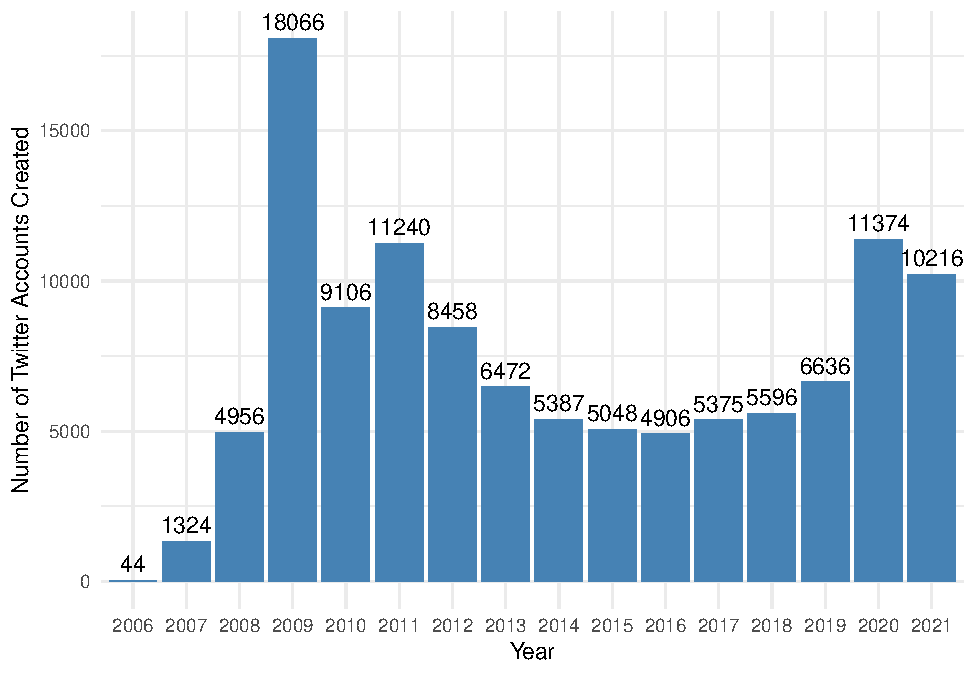
\includegraphics{Part_A_Tweets_files/figure-latex/number-of-twitter-accounts-1.pdf}

\subsubsection{Average Followers per
Year}\label{average-followers-per-year}

\begin{Shaded}
\begin{Highlighting}[]
\NormalTok{creators\_after\_2010 }\OtherTok{\textless{}{-}}\NormalTok{ tweets}
\NormalTok{creators\_after\_2010 }\OtherTok{\textless{}{-}}\NormalTok{ creators\_after\_2010 }\SpecialCharTok{\%\textgreater{}\%} \FunctionTok{mutate}\NormalTok{(}\AttributeTok{year =} \FunctionTok{as.numeric}\NormalTok{(}\FunctionTok{as.character}\NormalTok{(year)))}
\NormalTok{creators\_after\_2010 }\OtherTok{\textless{}{-}}\NormalTok{ creators\_after\_2010 }\SpecialCharTok{\%\textgreater{}\%} \FunctionTok{filter}\NormalTok{(year }\SpecialCharTok{\textgreater{}} \DecValTok{2010}\NormalTok{)}

\NormalTok{creators\_after\_2010 }\SpecialCharTok{\%\textgreater{}\%}
  \FunctionTok{filter}\NormalTok{(year }\SpecialCharTok{\textgreater{}} \DecValTok{2010}\NormalTok{) }\SpecialCharTok{\%\textgreater{}\%}
  \FunctionTok{group\_by}\NormalTok{(year) }\SpecialCharTok{\%\textgreater{}\%}
  \FunctionTok{summarise}\NormalTok{(}\AttributeTok{avg\_followers =} \FunctionTok{mean}\NormalTok{(user\_followers, }\AttributeTok{na.rm =} \ConstantTok{TRUE}\NormalTok{)) }\SpecialCharTok{\%\textgreater{}\%}
  \FunctionTok{ggplot}\NormalTok{(}\FunctionTok{aes}\NormalTok{(}\AttributeTok{x =}\NormalTok{ year, }\AttributeTok{y =}\NormalTok{ avg\_followers)) }\SpecialCharTok{+}
  \FunctionTok{geom\_bar}\NormalTok{(}\AttributeTok{stat =} \StringTok{"identity"}\NormalTok{, }\AttributeTok{fill =} \StringTok{"steelblue"}\NormalTok{) }\SpecialCharTok{+}
  \FunctionTok{geom\_text}\NormalTok{(}
    \FunctionTok{aes}\NormalTok{(}\AttributeTok{label =} \FunctionTok{round}\NormalTok{(avg\_followers, }\DecValTok{2}\NormalTok{)), }
    \AttributeTok{vjust =} \SpecialCharTok{{-}}\FloatTok{0.5}\NormalTok{) }\SpecialCharTok{+}
  \FunctionTok{scale\_x\_continuous}\NormalTok{(}\AttributeTok{breaks =}\NormalTok{ creators\_after\_2010}\SpecialCharTok{$}\NormalTok{year) }\SpecialCharTok{+}
  \FunctionTok{labs}\NormalTok{(}\AttributeTok{x =} \StringTok{"Year"}\NormalTok{, }\AttributeTok{y =} \StringTok{"Average Followers"}\NormalTok{) }\SpecialCharTok{+}
  \FunctionTok{theme\_minimal}\NormalTok{()}
\end{Highlighting}
\end{Shaded}

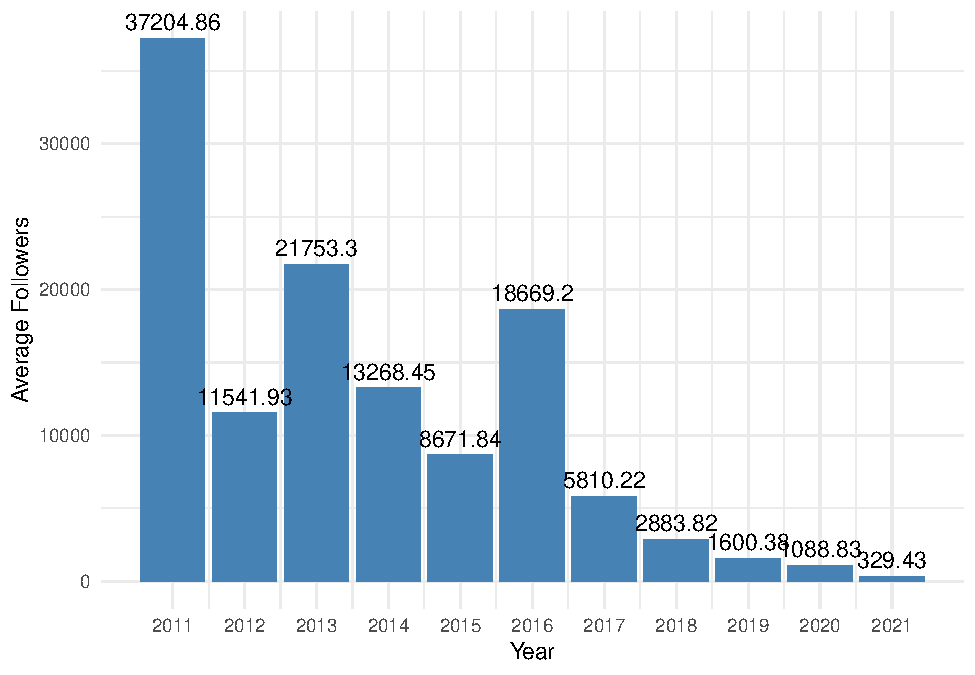
\includegraphics{Part_A_Tweets_files/figure-latex/average-followers-per-year-1.pdf}

\subsubsection{Top 10 Most Frequest Location of
Users}\label{top-10-most-frequest-location-of-users}

\begin{Shaded}
\begin{Highlighting}[]
\NormalTok{top\_locations }\OtherTok{\textless{}{-}}\NormalTok{ tweets }\SpecialCharTok{\%\textgreater{}\%}
  \FunctionTok{select}\NormalTok{(user\_screen\_name, user\_location) }\SpecialCharTok{\%\textgreater{}\%}
  \FunctionTok{distinct}\NormalTok{() }\SpecialCharTok{\%\textgreater{}\%}
  \FunctionTok{filter}\NormalTok{(}\SpecialCharTok{!}\FunctionTok{is.na}\NormalTok{(user\_location), user\_location }\SpecialCharTok{!=} \StringTok{""}\NormalTok{) }\SpecialCharTok{\%\textgreater{}\%}
  \FunctionTok{count}\NormalTok{(user\_location, }\AttributeTok{name=}\StringTok{"user\_count"}\NormalTok{) }\SpecialCharTok{\%\textgreater{}\%}
  \FunctionTok{arrange}\NormalTok{(}\FunctionTok{desc}\NormalTok{(user\_count)) }\SpecialCharTok{\%\textgreater{}\%}
\NormalTok{  dplyr}\SpecialCharTok{::}\FunctionTok{slice}\NormalTok{(}\DecValTok{1}\SpecialCharTok{:}\DecValTok{10}\NormalTok{)}

\NormalTok{top\_locations }\OtherTok{\textless{}{-}}\NormalTok{ top\_locations }\SpecialCharTok{\%\textgreater{}\%}
  \FunctionTok{mutate}\NormalTok{(}\AttributeTok{user\_location =} \FunctionTok{fct\_reorder}\NormalTok{(user\_location, user\_count, }\AttributeTok{.desc =} \ConstantTok{TRUE}\NormalTok{)) }\SpecialCharTok{\%\textgreater{}\%}
  \FunctionTok{mutate}\NormalTok{(}\AttributeTok{user\_location =} \FunctionTok{fct\_rev}\NormalTok{(user\_location))}

\FunctionTok{ggplot}\NormalTok{(top\_locations, }\FunctionTok{aes}\NormalTok{(}\AttributeTok{x =}\NormalTok{ user\_location, }\AttributeTok{y =}\NormalTok{ user\_count)) }\SpecialCharTok{+}
  \FunctionTok{geom\_col}\NormalTok{(}\AttributeTok{fill =} \StringTok{"steelblue"}\NormalTok{) }\SpecialCharTok{+}
  \FunctionTok{geom\_text}\NormalTok{(}\FunctionTok{aes}\NormalTok{(}\AttributeTok{label =}\NormalTok{ user\_count), }\AttributeTok{hjust =} \SpecialCharTok{{-}}\FloatTok{0.1}\NormalTok{, }\AttributeTok{vjust =} \FloatTok{0.5}\NormalTok{) }\SpecialCharTok{+}
  \FunctionTok{coord\_flip}\NormalTok{() }\SpecialCharTok{+}
  \FunctionTok{labs}\NormalTok{(}\AttributeTok{x =} \StringTok{"User Location"}\NormalTok{, }\AttributeTok{y =} \StringTok{"Number of Users"}\NormalTok{) }\SpecialCharTok{+}
  \FunctionTok{theme\_minimal}\NormalTok{() }\SpecialCharTok{+}
  \FunctionTok{scale\_y\_continuous}\NormalTok{(}\AttributeTok{expand =} \FunctionTok{expansion}\NormalTok{(}\AttributeTok{mult =} \FunctionTok{c}\NormalTok{(}\DecValTok{0}\NormalTok{, }\FloatTok{0.15}\NormalTok{)))}
\end{Highlighting}
\end{Shaded}

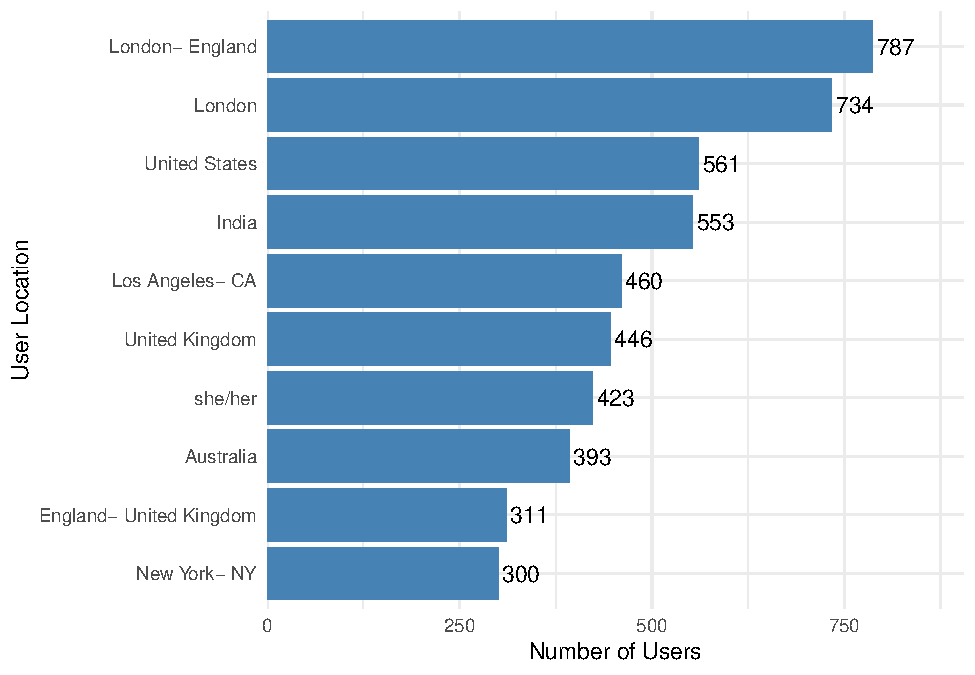
\includegraphics{Part_A_Tweets_files/figure-latex/top-10-most-frequent-location-1.pdf}

\subsubsection{Number of Tweets Associated with the Top 10
locations}\label{number-of-tweets-associated-with-the-top-10-locations}

\begin{Shaded}
\begin{Highlighting}[]
\NormalTok{tweets\_in\_top\_10\_locations }\OtherTok{\textless{}{-}}\NormalTok{ tweets }\SpecialCharTok{\%\textgreater{}\%}
  \FunctionTok{filter}\NormalTok{(user\_location }\SpecialCharTok{\%in\%}\NormalTok{ top\_locations}\SpecialCharTok{$}\NormalTok{user\_location) }\SpecialCharTok{\%\textgreater{}\%}
  \FunctionTok{group\_by}\NormalTok{(user\_location) }\SpecialCharTok{\%\textgreater{}\%}
  \FunctionTok{summarise}\NormalTok{(}\AttributeTok{tweet\_count =} \FunctionTok{n}\NormalTok{()) }\SpecialCharTok{\%\textgreater{}\%}
  \FunctionTok{arrange}\NormalTok{(}\FunctionTok{desc}\NormalTok{(tweet\_count))}

\NormalTok{tweets\_in\_top\_10\_locations }\OtherTok{\textless{}{-}}\NormalTok{ tweets\_in\_top\_10\_locations }\SpecialCharTok{\%\textgreater{}\%}
  \FunctionTok{mutate}\NormalTok{(}\AttributeTok{user\_location =} \FunctionTok{fct\_reorder}\NormalTok{(user\_location, tweet\_count, }\AttributeTok{.desc =} \ConstantTok{TRUE}\NormalTok{)) }\SpecialCharTok{\%\textgreater{}\%}
  \FunctionTok{mutate}\NormalTok{(}\AttributeTok{user\_location =} \FunctionTok{fct\_rev}\NormalTok{(user\_location))}

\FunctionTok{ggplot}\NormalTok{(tweets\_in\_top\_10\_locations, }\FunctionTok{aes}\NormalTok{(}\AttributeTok{x =}\NormalTok{ user\_location, }\AttributeTok{y =}\NormalTok{ tweet\_count)) }\SpecialCharTok{+}
  \FunctionTok{geom\_col}\NormalTok{(}\AttributeTok{fill =} \StringTok{"steelblue"}\NormalTok{) }\SpecialCharTok{+}
  \FunctionTok{geom\_text}\NormalTok{(}\FunctionTok{aes}\NormalTok{(}\AttributeTok{label =}\NormalTok{ tweet\_count), }\AttributeTok{hjust =} \SpecialCharTok{{-}}\FloatTok{0.1}\NormalTok{, }\AttributeTok{vjust =} \FloatTok{0.5}\NormalTok{) }\SpecialCharTok{+}
  \FunctionTok{coord\_flip}\NormalTok{() }\SpecialCharTok{+}
  \FunctionTok{labs}\NormalTok{(}\AttributeTok{x =} \StringTok{"User Location"}\NormalTok{, }\AttributeTok{y =} \StringTok{"Number of Tweets"}\NormalTok{) }\SpecialCharTok{+}
  \FunctionTok{theme\_minimal}\NormalTok{() }\SpecialCharTok{+}
  \FunctionTok{scale\_y\_continuous}\NormalTok{(}\AttributeTok{expand =} \FunctionTok{expansion}\NormalTok{(}\AttributeTok{mult =} \FunctionTok{c}\NormalTok{(}\DecValTok{0}\NormalTok{, }\FloatTok{0.15}\NormalTok{)))}
\end{Highlighting}
\end{Shaded}

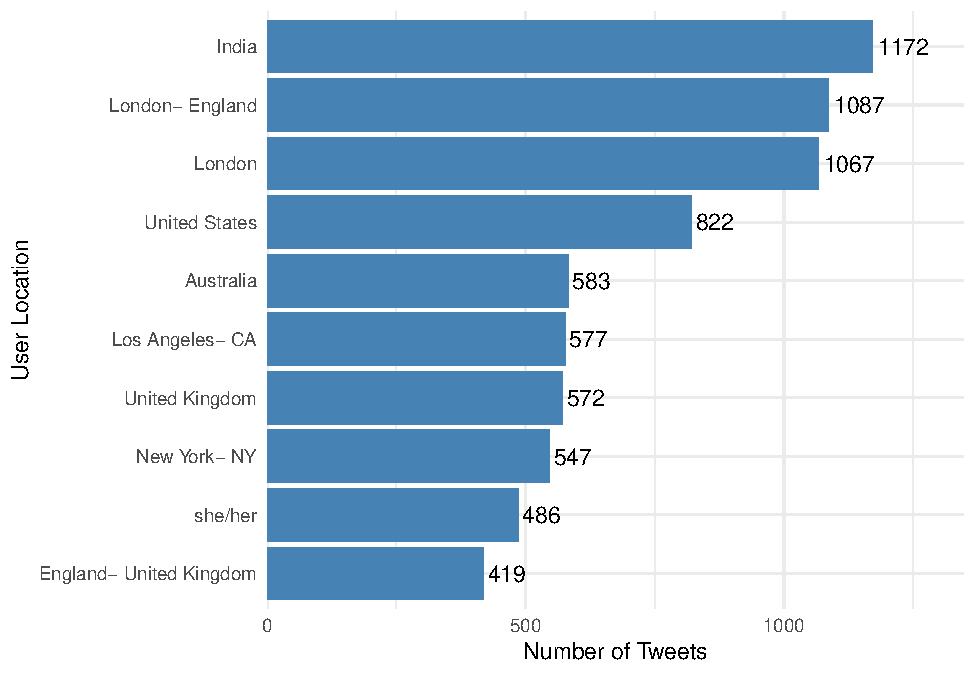
\includegraphics{Part_A_Tweets_files/figure-latex/number-of-tweets-associated-with-top-10-locations-1.pdf}

From the last two visualisations, the odd values are ``she/her'', and
some locations are the geographically the same from a broader
perspective, but some are more specific to cities. For example, ``New
York- NY'', ``Los Angeles- CA'', and ``United States''. The first two
locations are cities in the United States, but there is also ``United
States'' as a location.

\subsubsection{Bar Chart of the Length of
Tweets}\label{bar-chart-of-the-length-of-tweets}

\begin{Shaded}
\begin{Highlighting}[]
\NormalTok{tweets }\OtherTok{\textless{}{-}}\NormalTok{ tweets }\SpecialCharTok{\%\textgreater{}\%}
  \FunctionTok{mutate}\NormalTok{(}\AttributeTok{tweet\_length =} \FunctionTok{nchar}\NormalTok{(text)) }\SpecialCharTok{\%\textgreater{}\%}
  \FunctionTok{mutate}\NormalTok{(}\AttributeTok{length\_group =} \FunctionTok{case\_when}\NormalTok{(}
\NormalTok{    tweet\_length }\SpecialCharTok{\textgreater{}=} \DecValTok{1} \SpecialCharTok{\&}\NormalTok{ tweet\_length }\SpecialCharTok{\textless{}=} \DecValTok{40} \SpecialCharTok{\textasciitilde{}} \StringTok{"1{-}40"}\NormalTok{,}
\NormalTok{    tweet\_length }\SpecialCharTok{\textgreater{}=} \DecValTok{41} \SpecialCharTok{\&}\NormalTok{ tweet\_length }\SpecialCharTok{\textless{}=} \DecValTok{80} \SpecialCharTok{\textasciitilde{}} \StringTok{"41{-}80"}\NormalTok{,}
\NormalTok{    tweet\_length }\SpecialCharTok{\textgreater{}=} \DecValTok{81} \SpecialCharTok{\&}\NormalTok{ tweet\_length }\SpecialCharTok{\textless{}=} \DecValTok{120} \SpecialCharTok{\textasciitilde{}} \StringTok{"81{-}120"}\NormalTok{,}
\NormalTok{    tweet\_length }\SpecialCharTok{\textgreater{}=} \DecValTok{121} \SpecialCharTok{\&}\NormalTok{ tweet\_length }\SpecialCharTok{\textless{}=} \DecValTok{160} \SpecialCharTok{\textasciitilde{}} \StringTok{"121{-}160"}\NormalTok{,}
\NormalTok{    tweet\_length }\SpecialCharTok{\textgreater{}=} \DecValTok{161} \SpecialCharTok{\&}\NormalTok{ tweet\_length }\SpecialCharTok{\textless{}=} \DecValTok{200} \SpecialCharTok{\textasciitilde{}} \StringTok{"161{-}200"}\NormalTok{,}
\NormalTok{    tweet\_length }\SpecialCharTok{\textgreater{}=} \DecValTok{201} \SpecialCharTok{\&}\NormalTok{ tweet\_length }\SpecialCharTok{\textless{}=} \DecValTok{240} \SpecialCharTok{\textasciitilde{}} \StringTok{"201{-}240"}\NormalTok{,}
\NormalTok{    tweet\_length }\SpecialCharTok{\textgreater{}=} \DecValTok{241} \SpecialCharTok{\textasciitilde{}} \StringTok{"241+"}\NormalTok{,}
    \ConstantTok{TRUE} \SpecialCharTok{\textasciitilde{}} \StringTok{"Unknown"}
\NormalTok{  ))}

\NormalTok{length\_group\_counts }\OtherTok{\textless{}{-}}\NormalTok{ tweets }\SpecialCharTok{\%\textgreater{}\%}
  \FunctionTok{count}\NormalTok{(length\_group)}

\NormalTok{custom\_order }\OtherTok{\textless{}{-}} \FunctionTok{c}\NormalTok{(}\StringTok{"1{-}40"}\NormalTok{, }\StringTok{"41{-}80"}\NormalTok{, }\StringTok{"81{-}120"}\NormalTok{, }\StringTok{"121{-}160"}\NormalTok{, }\StringTok{"161{-}200"}\NormalTok{, }\StringTok{"201{-}240"}\NormalTok{, }\StringTok{"241+"}\NormalTok{)}
\NormalTok{length\_group\_counts }\OtherTok{\textless{}{-}}\NormalTok{ length\_group\_counts }\SpecialCharTok{\%\textgreater{}\%}
  \FunctionTok{mutate}\NormalTok{(}\AttributeTok{length\_group =} \FunctionTok{factor}\NormalTok{(length\_group, }\AttributeTok{levels =}\NormalTok{ custom\_order))}

\FunctionTok{ggplot}\NormalTok{(length\_group\_counts, }\FunctionTok{aes}\NormalTok{(}\AttributeTok{x =}\NormalTok{ length\_group, }\AttributeTok{y =}\NormalTok{ n)) }\SpecialCharTok{+}
  \FunctionTok{geom\_bar}\NormalTok{(}\AttributeTok{stat =} \StringTok{"identity"}\NormalTok{, }\AttributeTok{fill =} \StringTok{"steelblue"}\NormalTok{) }\SpecialCharTok{+}
  \FunctionTok{geom\_text}\NormalTok{(}\FunctionTok{aes}\NormalTok{(}\AttributeTok{label =}\NormalTok{ n), }\AttributeTok{vjust =} \SpecialCharTok{{-}}\FloatTok{0.5}\NormalTok{) }\SpecialCharTok{+}
  \FunctionTok{labs}\NormalTok{(}\AttributeTok{x =} \StringTok{"Length of Tweets"}\NormalTok{, }\AttributeTok{y =} \StringTok{"Number of Tweets"}\NormalTok{) }\SpecialCharTok{+}
  \FunctionTok{theme\_minimal}\NormalTok{()}
\end{Highlighting}
\end{Shaded}

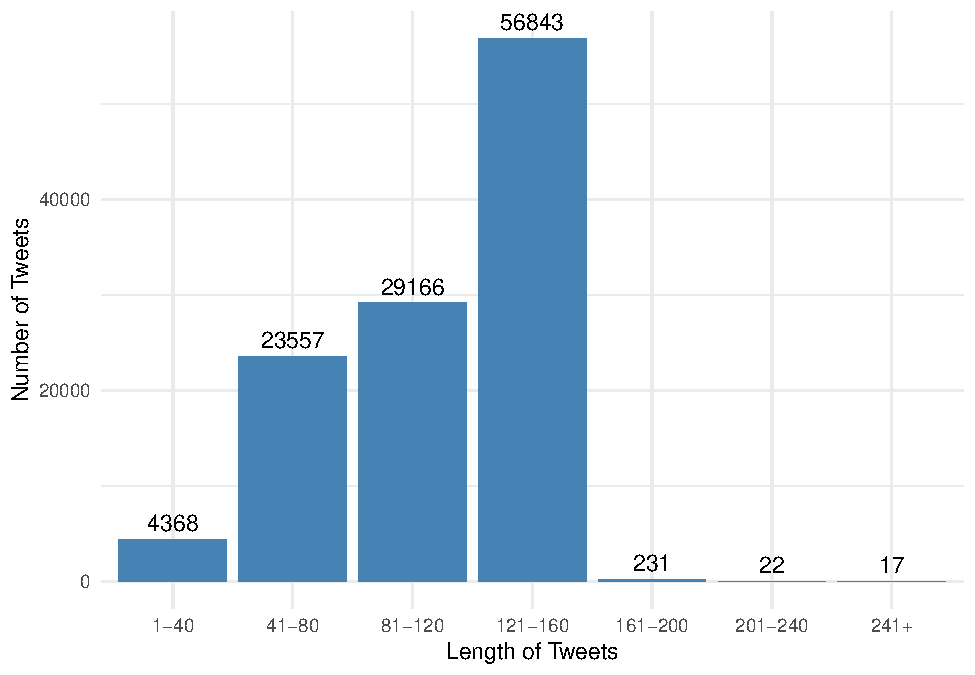
\includegraphics{Part_A_Tweets_files/figure-latex/bar-chart-of-length-of-tweets-1.pdf}

\subsubsection{Number of Tweets with Mentions and Its
Count}\label{number-of-tweets-with-mentions-and-its-count}

\begin{Shaded}
\begin{Highlighting}[]
\NormalTok{tweets\_with\_mentions }\OtherTok{\textless{}{-}}\NormalTok{ tweets }\SpecialCharTok{\%\textgreater{}\%}
  \FunctionTok{filter}\NormalTok{(}\FunctionTok{str\_detect}\NormalTok{(text, }\StringTok{"@[A{-}Za{-}z0{-}9\_]+"}\NormalTok{)) }\SpecialCharTok{\%\textgreater{}\%}
  \FunctionTok{mutate}\NormalTok{(}\AttributeTok{mentions\_count =} \FunctionTok{str\_count}\NormalTok{(text, }\StringTok{"@[A{-}Za{-}z0{-}9\_]+"}\NormalTok{))}

\NormalTok{tweets\_with\_mentions }\OtherTok{\textless{}{-}}\NormalTok{ tweets\_with\_mentions }\SpecialCharTok{\%\textgreater{}\%}
  \FunctionTok{group\_by}\NormalTok{(mentions\_count) }\SpecialCharTok{\%\textgreater{}\%}
  \FunctionTok{summarise}\NormalTok{(}\AttributeTok{tweet\_count =} \FunctionTok{n}\NormalTok{()) }\SpecialCharTok{\%\textgreater{}\%}
  \FunctionTok{arrange}\NormalTok{(}\FunctionTok{desc}\NormalTok{(tweet\_count))}

\NormalTok{tweets\_with\_mentions }\OtherTok{\textless{}{-}}\NormalTok{ tweets\_with\_mentions }\SpecialCharTok{\%\textgreater{}\%}
  \FunctionTok{mutate}\NormalTok{(}\AttributeTok{mentions\_count =} \FunctionTok{as.factor}\NormalTok{(mentions\_count)) }\SpecialCharTok{\%\textgreater{}\%}
  \FunctionTok{mutate}\NormalTok{(}\AttributeTok{mentions\_count =} \FunctionTok{fct\_reorder}\NormalTok{(mentions\_count, tweet\_count, }\AttributeTok{.desc =} \ConstantTok{TRUE}\NormalTok{)) }\SpecialCharTok{\%\textgreater{}\%}
  \FunctionTok{mutate}\NormalTok{(}\AttributeTok{mentions\_count =} \FunctionTok{fct\_rev}\NormalTok{(mentions\_count))}

\FunctionTok{ggplot}\NormalTok{(tweets\_with\_mentions, }\FunctionTok{aes}\NormalTok{(}\AttributeTok{x =}\NormalTok{ mentions\_count, }\AttributeTok{y =}\NormalTok{ tweet\_count)) }\SpecialCharTok{+}
  \FunctionTok{geom\_col}\NormalTok{(}\AttributeTok{fill =} \StringTok{"steelblue"}\NormalTok{) }\SpecialCharTok{+}
  \FunctionTok{coord\_flip}\NormalTok{() }\SpecialCharTok{+}
  \FunctionTok{geom\_text}\NormalTok{(}\FunctionTok{aes}\NormalTok{(}\AttributeTok{label =}\NormalTok{ tweet\_count), }\AttributeTok{hjust =} \SpecialCharTok{{-}}\FloatTok{0.1}\NormalTok{, }\AttributeTok{vjust =} \FloatTok{0.5}\NormalTok{) }\SpecialCharTok{+}
  \FunctionTok{labs}\NormalTok{(}\AttributeTok{x =} \StringTok{"Number of Mentions"}\NormalTok{, }\AttributeTok{y =} \StringTok{"Number of Tweets"}\NormalTok{) }\SpecialCharTok{+}
  \FunctionTok{theme\_minimal}\NormalTok{() }\SpecialCharTok{+}
  \FunctionTok{scale\_y\_continuous}\NormalTok{(}\AttributeTok{expand =} \FunctionTok{expansion}\NormalTok{(}\AttributeTok{mult =} \FunctionTok{c}\NormalTok{(}\DecValTok{0}\NormalTok{, }\FloatTok{0.15}\NormalTok{)))}
\end{Highlighting}
\end{Shaded}

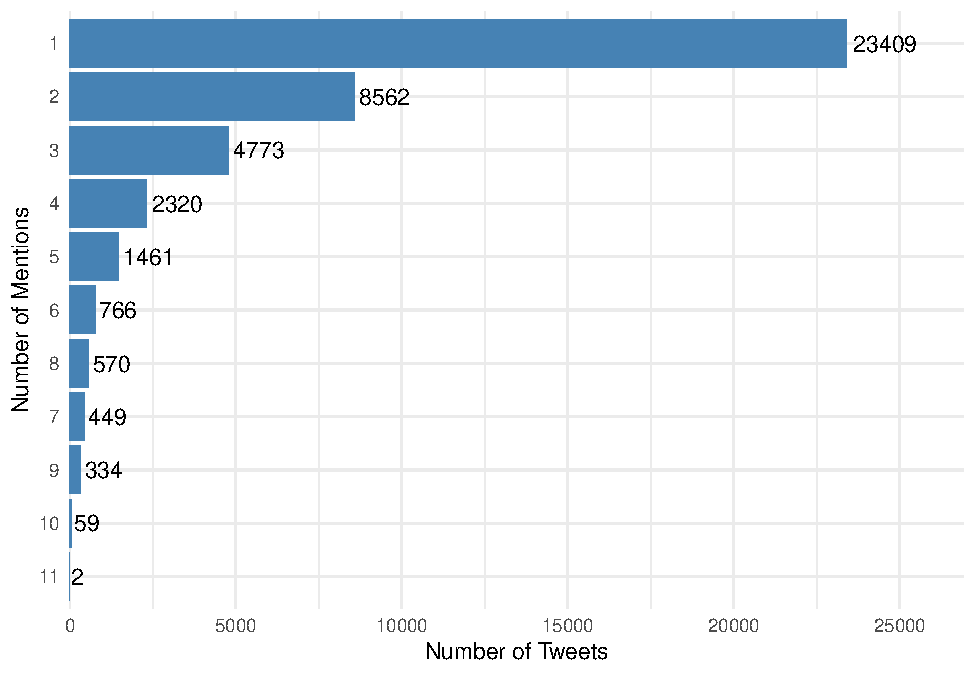
\includegraphics{Part_A_Tweets_files/figure-latex/number-of-tweets-with-mentions-1.pdf}

\begin{Shaded}
\begin{Highlighting}[]
\NormalTok{number\_of\_tweets\_with\_mentions }\OtherTok{\textless{}{-}}\NormalTok{ tweets }\SpecialCharTok{\%\textgreater{}\%}
  \FunctionTok{filter}\NormalTok{(}\FunctionTok{str\_detect}\NormalTok{(text, }\StringTok{"@[A{-}Za{-}z0{-}9\_]+"}\NormalTok{)) }\SpecialCharTok{\%\textgreater{}\%}
  \FunctionTok{nrow}\NormalTok{()}

\NormalTok{number\_of\_tweets\_with\_3\_or\_more\_mentions }\OtherTok{\textless{}{-}}\NormalTok{ tweets }\SpecialCharTok{\%\textgreater{}\%}
  \FunctionTok{filter}\NormalTok{(}\FunctionTok{str\_detect}\NormalTok{(text, }\StringTok{"@[A{-}Za{-}z0{-}9\_]+"}\NormalTok{)) }\SpecialCharTok{\%\textgreater{}\%}
  \FunctionTok{mutate}\NormalTok{(}\AttributeTok{mentions\_count =} \FunctionTok{str\_count}\NormalTok{(text, }\StringTok{"@[A{-}Za{-}z0{-}9\_]+"}\NormalTok{)) }\SpecialCharTok{\%\textgreater{}\%}
  \FunctionTok{filter}\NormalTok{(mentions\_count }\SpecialCharTok{\textgreater{}=} \DecValTok{3}\NormalTok{) }\SpecialCharTok{\%\textgreater{}\%}
  \FunctionTok{nrow}\NormalTok{()}

\FunctionTok{cat}\NormalTok{(}\StringTok{"Number of tweets with mentions: "}\NormalTok{, number\_of\_tweets\_with\_mentions, }\StringTok{"}\SpecialCharTok{\textbackslash{}n}\StringTok{"}\NormalTok{)}
\end{Highlighting}
\end{Shaded}

\begin{verbatim}
## Number of tweets with mentions:  42705
\end{verbatim}

\begin{Shaded}
\begin{Highlighting}[]
\FunctionTok{cat}\NormalTok{(}\StringTok{"Number of tweets with 3 or more mentions: "}\NormalTok{, number\_of\_tweets\_with\_3\_or\_more\_mentions, }\StringTok{"}\SpecialCharTok{\textbackslash{}n}\StringTok{"}\NormalTok{)}
\end{Highlighting}
\end{Shaded}

\begin{verbatim}
## Number of tweets with 3 or more mentions:  10734
\end{verbatim}

\subsubsection{Top 20 Most Frequent Term in
Tweets}\label{top-20-most-frequent-term-in-tweets}

\begin{Shaded}
\begin{Highlighting}[]
\FunctionTok{library}\NormalTok{(tidytext)}

\NormalTok{tweets\_frequent\_terms }\OtherTok{\textless{}{-}}\NormalTok{ tweets }\SpecialCharTok{\%\textgreater{}\%}
  \FunctionTok{mutate}\NormalTok{(}\AttributeTok{text =} \FunctionTok{tolower}\NormalTok{(text)) }\SpecialCharTok{\%\textgreater{}\%}
  \FunctionTok{unnest\_tokens}\NormalTok{(word, text) }\SpecialCharTok{\%\textgreater{}\%}
  \FunctionTok{count}\NormalTok{(word, }\AttributeTok{sort =} \ConstantTok{TRUE}\NormalTok{)}

\NormalTok{top\_20\_terms }\OtherTok{\textless{}{-}}\NormalTok{ tweets\_frequent\_terms }\SpecialCharTok{\%\textgreater{}\%}
\NormalTok{  dplyr}\SpecialCharTok{::}\FunctionTok{slice}\NormalTok{(}\DecValTok{1}\SpecialCharTok{:}\DecValTok{20}\NormalTok{) }\SpecialCharTok{\%\textgreater{}\%}
  \FunctionTok{mutate}\NormalTok{(}\AttributeTok{word =} \FunctionTok{fct\_reorder}\NormalTok{(word, n)) }\SpecialCharTok{\%\textgreater{}\%}
  \FunctionTok{mutate}\NormalTok{(}\AttributeTok{word =} \FunctionTok{fct\_rev}\NormalTok{(word))}

\NormalTok{max\_count }\OtherTok{\textless{}{-}} \FunctionTok{max}\NormalTok{(top\_20\_terms}\SpecialCharTok{$}\NormalTok{n)}

\FunctionTok{ggplot}\NormalTok{(top\_20\_terms, }\FunctionTok{aes}\NormalTok{(}\AttributeTok{x =} \FunctionTok{reorder}\NormalTok{(word, n), }\AttributeTok{y =}\NormalTok{ n)) }\SpecialCharTok{+}
  \FunctionTok{geom\_col}\NormalTok{(}\AttributeTok{fill =} \StringTok{"steelblue"}\NormalTok{) }\SpecialCharTok{+}
  \FunctionTok{geom\_text}\NormalTok{(}\FunctionTok{aes}\NormalTok{(}\AttributeTok{label =}\NormalTok{ n), }\AttributeTok{hjust =} \SpecialCharTok{{-}}\FloatTok{0.1}\NormalTok{, }\AttributeTok{vjust =} \FloatTok{0.5}\NormalTok{) }\SpecialCharTok{+}
  \FunctionTok{coord\_flip}\NormalTok{() }\SpecialCharTok{+}
  \FunctionTok{labs}\NormalTok{(}\AttributeTok{x =} \StringTok{"Word"}\NormalTok{, }\AttributeTok{y =} \StringTok{"Number of Occurrences"}\NormalTok{) }\SpecialCharTok{+}
  \FunctionTok{theme\_minimal}\NormalTok{() }\SpecialCharTok{+}
  \FunctionTok{scale\_y\_continuous}\NormalTok{(}\AttributeTok{expand =} \FunctionTok{expansion}\NormalTok{(}\AttributeTok{mult =} \FunctionTok{c}\NormalTok{(}\DecValTok{0}\NormalTok{, }\FloatTok{0.15}\NormalTok{)))}
\end{Highlighting}
\end{Shaded}

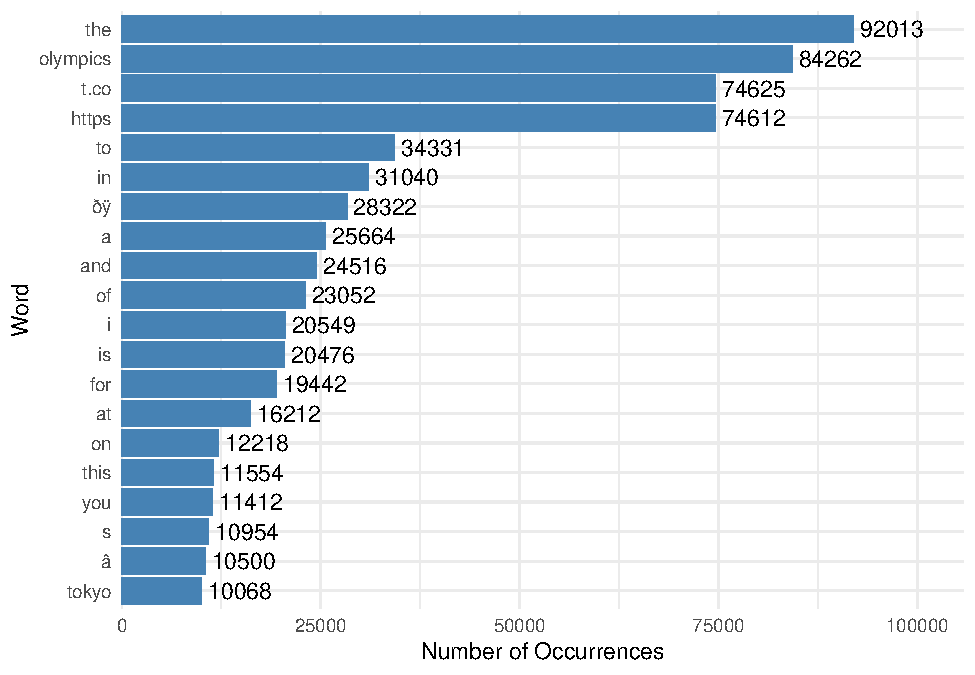
\includegraphics{Part_A_Tweets_files/figure-latex/top-20-most-frequent-terms-1.pdf}

\subsubsection{Top 20 Most Frequent Non-Stopword Term in
Tweets}\label{top-20-most-frequent-non-stopword-term-in-tweets}

\begin{Shaded}
\begin{Highlighting}[]
\NormalTok{tweets\_frequent\_terms\_no\_stopwords }\OtherTok{\textless{}{-}}\NormalTok{ tweets }\SpecialCharTok{\%\textgreater{}\%}
  \FunctionTok{mutate}\NormalTok{(}\AttributeTok{text =} \FunctionTok{tolower}\NormalTok{(text)) }\SpecialCharTok{\%\textgreater{}\%}
  \FunctionTok{unnest\_tokens}\NormalTok{(word, text) }\SpecialCharTok{\%\textgreater{}\%}
  \FunctionTok{anti\_join}\NormalTok{(stop\_words) }\SpecialCharTok{\%\textgreater{}\%}
  \FunctionTok{count}\NormalTok{(word, }\AttributeTok{sort =} \ConstantTok{TRUE}\NormalTok{)}

\NormalTok{top\_20\_terms\_no\_stopwords }\OtherTok{\textless{}{-}}\NormalTok{ tweets\_frequent\_terms\_no\_stopwords }\SpecialCharTok{\%\textgreater{}\%}
\NormalTok{  dplyr}\SpecialCharTok{::}\FunctionTok{slice}\NormalTok{(}\DecValTok{1}\SpecialCharTok{:}\DecValTok{20}\NormalTok{) }\SpecialCharTok{\%\textgreater{}\%}
  \FunctionTok{mutate}\NormalTok{(}\AttributeTok{word =} \FunctionTok{fct\_reorder}\NormalTok{(word, n)) }\SpecialCharTok{\%\textgreater{}\%}
  \FunctionTok{mutate}\NormalTok{(}\AttributeTok{word =} \FunctionTok{fct\_rev}\NormalTok{(word))}

\NormalTok{max\_count\_no\_stopwords }\OtherTok{\textless{}{-}} \FunctionTok{max}\NormalTok{(top\_20\_terms\_no\_stopwords}\SpecialCharTok{$}\NormalTok{n)}

\FunctionTok{ggplot}\NormalTok{(top\_20\_terms\_no\_stopwords, }\FunctionTok{aes}\NormalTok{(}\AttributeTok{x =} \FunctionTok{reorder}\NormalTok{(word, n), }\AttributeTok{y =}\NormalTok{ n)) }\SpecialCharTok{+}
  \FunctionTok{geom\_col}\NormalTok{(}\AttributeTok{fill =} \StringTok{"steelblue"}\NormalTok{) }\SpecialCharTok{+}
  \FunctionTok{geom\_text}\NormalTok{(}\FunctionTok{aes}\NormalTok{(}\AttributeTok{label =}\NormalTok{ n), }\AttributeTok{hjust =} \SpecialCharTok{{-}}\FloatTok{0.1}\NormalTok{, }\AttributeTok{vjust =} \FloatTok{0.5}\NormalTok{) }\SpecialCharTok{+}
  \FunctionTok{coord\_flip}\NormalTok{() }\SpecialCharTok{+}
  \FunctionTok{labs}\NormalTok{(}\AttributeTok{x =} \StringTok{"Word"}\NormalTok{, }\AttributeTok{y =} \StringTok{"Number of Occurrences"}\NormalTok{) }\SpecialCharTok{+}
  \FunctionTok{theme\_minimal}\NormalTok{() }\SpecialCharTok{+}
  \FunctionTok{scale\_y\_continuous}\NormalTok{(}\AttributeTok{expand =} \FunctionTok{expansion}\NormalTok{(}\AttributeTok{mult =} \FunctionTok{c}\NormalTok{(}\DecValTok{0}\NormalTok{, }\FloatTok{0.15}\NormalTok{)))}
\end{Highlighting}
\end{Shaded}

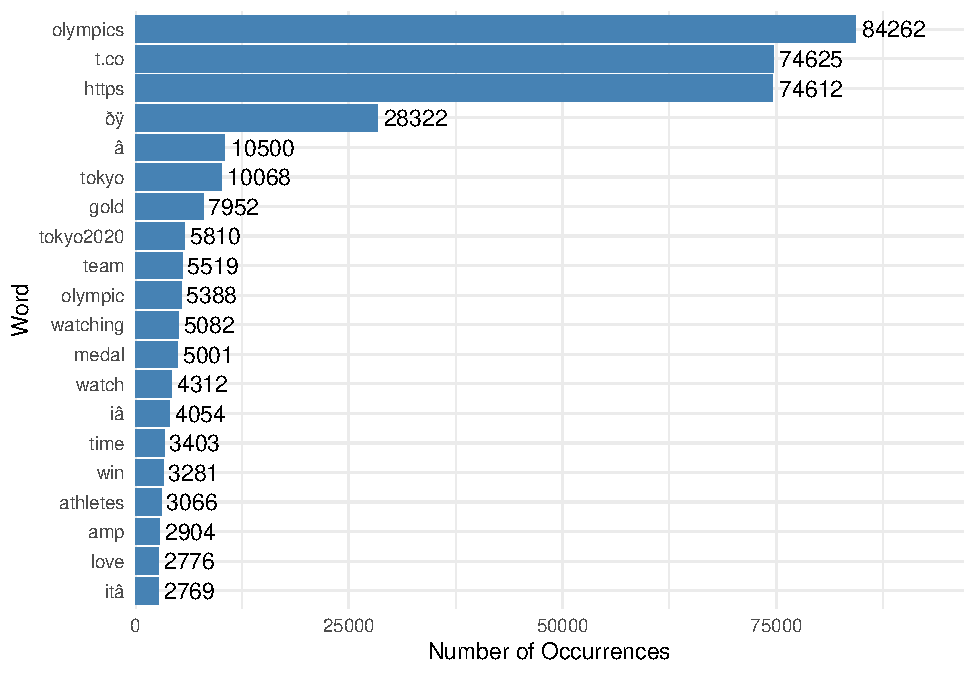
\includegraphics{Part_A_Tweets_files/figure-latex/top-20-most-frequent-terms-with-no-stopwords-1.pdf}
\vspace{2cm}

\section{Predictive Data Analysis}\label{predictive-data-analysis}

\subsection{Model Training}\label{model-training}

In this section, I will build machine learning models to predict whether
a tweet is relevant or not. I will use the glm function to build a
logistic regression models using all of the features from the dataset.
The glm function is used to fit generalized linear models, which can be
used for binary classification tasks like this one. Next, I will try to
use interaction terms to see if that can improve the same model's
performance. FInally, I will use the xgboost package to build a gradient
boosting model to also evaluate how it performs compared to the logistic
regression models.

First, I will make sure that the dependent variable is numeric and has
only two values, 0 and 1. Luckily, the dataset has already been split
into training and testing sets, so I will use the training set to build
the models and the testing set to evaluate them.

\begin{Shaded}
\begin{Highlighting}[]
\CommentTok{\# Load the training and testing datasets}
\NormalTok{train }\OtherTok{\textless{}{-}} \FunctionTok{read.csv}\NormalTok{(}\StringTok{"predictive\_twitter\_train.csv"}\NormalTok{)}

\CommentTok{\# Check missing values in relevanceJudge column}
\FunctionTok{cat}\NormalTok{(}\StringTok{"Missing values in relevanceJudge column: "}\NormalTok{, }
    \FunctionTok{sum}\NormalTok{(}\FunctionTok{is.na}\NormalTok{(train}\SpecialCharTok{$}\NormalTok{relevanceJudge)), }\StringTok{"}\SpecialCharTok{\textbackslash{}n}\StringTok{"}\NormalTok{)}
\end{Highlighting}
\end{Shaded}

\begin{verbatim}
## Missing values in relevanceJudge column:  0
\end{verbatim}

\begin{Shaded}
\begin{Highlighting}[]
\CommentTok{\# Check if relevanceJudge is numeric}
\FunctionTok{cat}\NormalTok{(}\StringTok{"Is relevanceJudge numeric: "}\NormalTok{, }
    \FunctionTok{is.numeric}\NormalTok{(train}\SpecialCharTok{$}\NormalTok{relevanceJudge), }\StringTok{"}\SpecialCharTok{\textbackslash{}n}\StringTok{"}\NormalTok{)}
\end{Highlighting}
\end{Shaded}

\begin{verbatim}
## Is relevanceJudge numeric:  TRUE
\end{verbatim}

\begin{Shaded}
\begin{Highlighting}[]
\CommentTok{\# Number of columns in the training set}
\FunctionTok{cat}\NormalTok{(}\StringTok{"Number of columns in the training set: "}\NormalTok{, }
    \FunctionTok{ncol}\NormalTok{(train), }\StringTok{"}\SpecialCharTok{\textbackslash{}n}\StringTok{"}\NormalTok{)}
\end{Highlighting}
\end{Shaded}

\begin{verbatim}
## Number of columns in the training set:  26
\end{verbatim}

\begin{Shaded}
\begin{Highlighting}[]
\CommentTok{\# Number of columns that are numeric in the training set}
\FunctionTok{cat}\NormalTok{(}\StringTok{"Number of numeric columns in the training set: "}\NormalTok{, }
    \FunctionTok{sum}\NormalTok{(}\FunctionTok{sapply}\NormalTok{(train, is.numeric)), }\StringTok{"}\SpecialCharTok{\textbackslash{}n}\StringTok{"}\NormalTok{)}
\end{Highlighting}
\end{Shaded}

\begin{verbatim}
## Number of numeric columns in the training set:  26
\end{verbatim}

\begin{Shaded}
\begin{Highlighting}[]
\CommentTok{\# Exclude tweetID from the training set}
\NormalTok{train }\OtherTok{\textless{}{-}}\NormalTok{ train }\SpecialCharTok{\%\textgreater{}\%}
  \FunctionTok{select}\NormalTok{(}\SpecialCharTok{{-}}\NormalTok{tweetID)}

\CommentTok{\# Rename mistakenly named column nFavorties to nFavorites}
\NormalTok{train }\OtherTok{\textless{}{-}}\NormalTok{ train }\SpecialCharTok{\%\textgreater{}\%}
  \FunctionTok{rename}\NormalTok{(}\AttributeTok{nFavorites =}\NormalTok{ nFavorties)}
\end{Highlighting}
\end{Shaded}

From the output in the code chunk above, we can see that the
\texttt{relevanceJudge} column has no missing values, is numeric, and
there are 26 columns in the training set, all of which are numeric.
Next, I will build a logistic regression model using the \texttt{glm}
function. I will use the \texttt{relevanceJudge} column as the dependent
variable and all other columns as independent variables.

\begin{Shaded}
\begin{Highlighting}[]
\CommentTok{\# Build the logistic regression model}
\NormalTok{model1 }\OtherTok{\textless{}{-}} \FunctionTok{glm}\NormalTok{(relevanceJudge }\SpecialCharTok{\textasciitilde{}}\NormalTok{ ., }\AttributeTok{data =}\NormalTok{ train, }\AttributeTok{family =}\NormalTok{ binomial)}

\CommentTok{\# Summary of the model}
\FunctionTok{summary}\NormalTok{(model1)}
\end{Highlighting}
\end{Shaded}

\begin{verbatim}
## 
## Call:
## glm(formula = relevanceJudge ~ ., family = binomial, data = train)
## 
## Coefficients:
##                         Estimate Std. Error z value Pr(>|z|)    
## (Intercept)           -4.235e-01  1.332e-01  -3.178 0.001481 ** 
## text_score             1.778e-01  1.414e-02  12.569  < 2e-16 ***
## text_score_expansion   1.001e-01  1.340e-02   7.467 8.23e-14 ***
## hashtag                7.541e-02  5.716e-02   1.319 0.187098    
## hasURL                 1.195e+00  5.882e-02  20.321  < 2e-16 ***
## isReply               -7.550e-01  1.237e-01  -6.105 1.03e-09 ***
## length                 2.036e-04  7.731e-04   0.263 0.792248    
## tweet_topic_time_diff -9.101e-03  5.197e-03  -1.751 0.079929 .  
## semantic_overlap       9.292e-01  6.234e-02  14.905  < 2e-16 ***
## X.entityTypes          2.788e-01  6.843e-02   4.074 4.62e-05 ***
## X.entities             3.973e-02  1.778e-02   2.234 0.025489 *  
## organization_entities -1.462e-01  6.233e-02  -2.345 0.019019 *  
## person_entities       -1.279e-01  6.132e-02  -2.087 0.036926 *  
## work_entities         -4.053e-01  7.101e-02  -5.708 1.14e-08 ***
## event_entities        -2.652e+00  7.210e-01  -3.678 0.000235 ***
## species_entities      -8.771e-01  3.137e-01  -2.796 0.005170 ** 
## places_entities       -1.307e-01  6.412e-02  -2.039 0.041453 *  
## nFollowers            -2.921e-06  1.337e-06  -2.185 0.028874 *  
## nFriends               6.504e-06  3.846e-06   1.691 0.090849 .  
## nFavorites             2.204e-06  6.977e-06   0.316 0.752098    
## nListed                9.748e-05  4.444e-05   2.193 0.028285 *  
## isVerified             7.840e-01  2.594e-01   3.023 0.002506 ** 
## isGeoEnabled           1.067e-02  5.493e-02   0.194 0.845962    
## twitterAge             1.672e-01  2.599e-02   6.434 1.24e-10 ***
## X.tweetsPosted        -1.664e-06  4.380e-07  -3.799 0.000146 ***
## ---
## Signif. codes:  0 '***' 0.001 '**' 0.01 '*' 0.05 '.' 0.1 ' ' 1
## 
## (Dispersion parameter for binomial family taken to be 1)
## 
##     Null deviance: 18338  on 35846  degrees of freedom
## Residual deviance: 14354  on 35822  degrees of freedom
##   (112 observations deleted due to missingness)
## AIC: 14404
## 
## Number of Fisher Scoring iterations: 7
\end{verbatim}

\begin{Shaded}
\begin{Highlighting}[]
\CommentTok{\# Check the coefficients of the model}
\FunctionTok{cat}\NormalTok{(}\StringTok{"Coefficients of the model with all of the features: }\SpecialCharTok{\textbackslash{}n}\StringTok{"}\NormalTok{)}
\end{Highlighting}
\end{Shaded}

\begin{verbatim}
## Coefficients of the model with all of the features:
\end{verbatim}

\begin{Shaded}
\begin{Highlighting}[]
\FunctionTok{print}\NormalTok{(}\FunctionTok{coef}\NormalTok{(model1))}
\end{Highlighting}
\end{Shaded}

\begin{verbatim}
##           (Intercept)            text_score  text_score_expansion 
##         -4.235116e-01          1.777828e-01          1.000739e-01 
##               hashtag                hasURL               isReply 
##          7.541028e-02          1.195298e+00         -7.549720e-01 
##                length tweet_topic_time_diff      semantic_overlap 
##          2.036337e-04         -9.101056e-03          9.292260e-01 
##         X.entityTypes            X.entities organization_entities 
##          2.787911e-01          3.973013e-02         -1.461808e-01 
##       person_entities         work_entities        event_entities 
##         -1.279425e-01         -4.053250e-01         -2.651862e+00 
##      species_entities       places_entities            nFollowers 
##         -8.771407e-01         -1.307291e-01         -2.921211e-06 
##              nFriends            nFavorites               nListed 
##          6.503686e-06          2.203739e-06          9.747565e-05 
##            isVerified          isGeoEnabled            twitterAge 
##          7.839781e-01          1.067119e-02          1.672066e-01 
##        X.tweetsPosted 
##         -1.663699e-06
\end{verbatim}

Next, I will build another model with interaction terms between some of
the author's account details.

\begin{Shaded}
\begin{Highlighting}[]
\CommentTok{\# Build the logistic regression model with interaction terms}
\NormalTok{model2 }\OtherTok{\textless{}{-}} \FunctionTok{glm}\NormalTok{(relevanceJudge }\SpecialCharTok{\textasciitilde{}}\NormalTok{ isVerified }\SpecialCharTok{*}
\NormalTok{              nFollowers }\SpecialCharTok{*}
\NormalTok{              nFriends }\SpecialCharTok{*}
\NormalTok{              nFavorites }\SpecialCharTok{*}
\NormalTok{              nListed }\SpecialCharTok{+}
\NormalTok{              .,}
              \AttributeTok{data =}\NormalTok{ train, }\AttributeTok{family =}\NormalTok{ binomial)}

\CommentTok{\# Summary of the model}
\FunctionTok{summary}\NormalTok{(model2)}
\end{Highlighting}
\end{Shaded}

\begin{verbatim}
## 
## Call:
## glm(formula = relevanceJudge ~ isVerified * nFollowers * nFriends * 
##     nFavorites * nListed + ., family = binomial, data = train)
## 
## Coefficients:
##                                                     Estimate Std. Error
## (Intercept)                                       -2.001e+15  2.324e+06
## isVerified                                         3.659e+14  6.647e+06
## nFollowers                                        -3.262e+09  3.691e+01
## nFriends                                           8.710e+08  1.722e+02
## nFavorites                                         8.264e+09  3.544e+02
## nListed                                            1.140e+11  1.847e+03
## text_score                                         1.266e+13  2.605e+05
## text_score_expansion                              -4.175e+13  2.446e+05
## hashtag                                            6.350e+13  9.147e+05
## hasURL                                             3.905e+14  7.981e+05
## isReply                                           -5.003e+14  1.135e+06
## length                                             9.043e+11  1.113e+04
## tweet_topic_time_diff                             -5.086e+12  8.387e+04
## semantic_overlap                                   7.829e+14  1.600e+06
## X.entityTypes                                      1.392e+14  1.113e+06
## X.entities                                         2.752e+13  2.889e+05
## organization_entities                             -7.449e+13  1.072e+06
## person_entities                                   -7.642e+13  1.038e+06
## work_entities                                     -2.155e+14  9.700e+05
## event_entities                                    -2.775e+15  5.325e+06
## species_entities                                  -3.476e+14  2.993e+06
## places_entities                                   -1.048e+14  1.101e+06
## isGeoEnabled                                       2.609e+13  8.423e+05
## twitterAge                                         7.114e+13  4.193e+05
## X.tweetsPosted                                    -5.089e+08  6.484e+00
## isVerified:nFollowers                              3.437e+09  3.997e+01
## isVerified:nFriends                                1.352e+10  1.683e+03
## nFollowers:nFriends                               -4.900e+04  2.446e-03
## isVerified:nFavorites                             -4.304e+11  1.265e+04
## nFollowers:nFavorites                              1.423e+06  4.601e-02
## nFriends:nFavorites                               -4.262e+06  1.066e-01
## isVerified:nListed                                -1.132e+11  2.052e+03
## nFollowers:nListed                                -6.598e+04  1.308e-03
## nFriends:nListed                                  -4.837e+05  1.350e-01
## nFavorites:nListed                                -1.420e+07  4.496e-01
## isVerified:nFollowers:nFriends                    -4.276e+05  5.439e-03
## isVerified:nFollowers:nFavorites                  -1.025e+07  2.281e-01
## isVerified:nFriends:nFavorites                     7.432e+07  9.445e+00
## nFollowers:nFriends:nFavorites                     5.028e+01  1.341e-06
## isVerified:nFollowers:nListed                      5.328e+04  1.336e-03
## isVerified:nFriends:nListed                        1.384e+07  2.905e-01
## nFollowers:nFriends:nListed                        3.158e+01  8.185e-07
## isVerified:nFavorites:nListed                      2.114e+08  8.324e+00
## nFollowers:nFavorites:nListed                     -3.186e+02  1.005e-05
## nFriends:nFavorites:nListed                        3.824e+03  1.180e-04
## isVerified:nFollowers:nFriends:nFavorites         -1.693e+02  6.038e-05
## isVerified:nFollowers:nFriends:nListed            -2.219e+01  8.612e-07
## isVerified:nFollowers:nFavorites:nListed           6.118e+02  1.346e-05
## isVerified:nFriends:nFavorites:nListed            -2.775e+04  9.404e-04
## nFollowers:nFriends:nFavorites:nListed            -5.248e-02  1.204e-09
## isVerified:nFollowers:nFriends:nFavorites:nListed  9.821e-02  3.559e-09
##                                                      z value Pr(>|z|)    
## (Intercept)                                       -861014825   <2e-16 ***
## isVerified                                          55041097   <2e-16 ***
## nFollowers                                         -88376849   <2e-16 ***
## nFriends                                             5057530   <2e-16 ***
## nFavorites                                          23320687   <2e-16 ***
## nListed                                             61755358   <2e-16 ***
## text_score                                          48596580   <2e-16 ***
## text_score_expansion                              -170697179   <2e-16 ***
## hashtag                                             69426817   <2e-16 ***
## hasURL                                             489279939   <2e-16 ***
## isReply                                           -440820538   <2e-16 ***
## length                                              81213733   <2e-16 ***
## tweet_topic_time_diff                              -60642376   <2e-16 ***
## semantic_overlap                                   489223003   <2e-16 ***
## X.entityTypes                                      125121068   <2e-16 ***
## X.entities                                          95239214   <2e-16 ***
## organization_entities                              -69465694   <2e-16 ***
## person_entities                                    -73589546   <2e-16 ***
## work_entities                                     -222127214   <2e-16 ***
## event_entities                                    -521171025   <2e-16 ***
## species_entities                                  -116130170   <2e-16 ***
## places_entities                                    -95130244   <2e-16 ***
## isGeoEnabled                                        30970959   <2e-16 ***
## twitterAge                                         169654654   <2e-16 ***
## X.tweetsPosted                                     -78479908   <2e-16 ***
## isVerified:nFollowers                               85987831   <2e-16 ***
## isVerified:nFriends                                  8033818   <2e-16 ***
## nFollowers:nFriends                                -20031292   <2e-16 ***
## isVerified:nFavorites                              -34018918   <2e-16 ***
## nFollowers:nFavorites                               30939253   <2e-16 ***
## nFriends:nFavorites                                -39987431   <2e-16 ***
## isVerified:nListed                                 -55178701   <2e-16 ***
## nFollowers:nListed                                 -50458594   <2e-16 ***
## nFriends:nListed                                    -3583594   <2e-16 ***
## nFavorites:nListed                                 -31580848   <2e-16 ***
## isVerified:nFollowers:nFriends                     -78619672   <2e-16 ***
## isVerified:nFollowers:nFavorites                   -44929033   <2e-16 ***
## isVerified:nFriends:nFavorites                       7869117   <2e-16 ***
## nFollowers:nFriends:nFavorites                      37503540   <2e-16 ***
## isVerified:nFollowers:nListed                       39891051   <2e-16 ***
## isVerified:nFriends:nListed                         47647445   <2e-16 ***
## nFollowers:nFriends:nListed                         38576780   <2e-16 ***
## isVerified:nFavorites:nListed                       25396917   <2e-16 ***
## nFollowers:nFavorites:nListed                      -31708131   <2e-16 ***
## nFriends:nFavorites:nListed                         32414860   <2e-16 ***
## isVerified:nFollowers:nFriends:nFavorites           -2804761   <2e-16 ***
## isVerified:nFollowers:nFriends:nListed             -25762649   <2e-16 ***
## isVerified:nFollowers:nFavorites:nListed            45445230   <2e-16 ***
## isVerified:nFriends:nFavorites:nListed             -29505961   <2e-16 ***
## nFollowers:nFriends:nFavorites:nListed             -43586628   <2e-16 ***
## isVerified:nFollowers:nFriends:nFavorites:nListed   27591854   <2e-16 ***
## ---
## Signif. codes:  0 '***' 0.001 '**' 0.01 '*' 0.05 '.' 0.1 ' ' 1
## 
## (Dispersion parameter for binomial family taken to be 1)
## 
##     Null deviance:  18338  on 35846  degrees of freedom
## Residual deviance: 187283  on 35796  degrees of freedom
##   (112 observations deleted due to missingness)
## AIC: 187385
## 
## Number of Fisher Scoring iterations: 25
\end{verbatim}

\begin{Shaded}
\begin{Highlighting}[]
\CommentTok{\# Check the coefficients of the model}
\FunctionTok{cat}\NormalTok{(}\StringTok{"Coefficients of the model with interaction terms:}\SpecialCharTok{\textbackslash{}n}\StringTok{"}\NormalTok{)}
\end{Highlighting}
\end{Shaded}

\begin{verbatim}
## Coefficients of the model with interaction terms:
\end{verbatim}

\begin{Shaded}
\begin{Highlighting}[]
\FunctionTok{print}\NormalTok{(}\FunctionTok{coef}\NormalTok{(model2))}
\end{Highlighting}
\end{Shaded}

\begin{verbatim}
##                                       (Intercept) 
##                                     -2.001074e+15 
##                                        isVerified 
##                                      3.658789e+14 
##                                        nFollowers 
##                                     -3.261598e+09 
##                                          nFriends 
##                                      8.710216e+08 
##                                        nFavorites 
##                                      8.264190e+09 
##                                           nListed 
##                                      1.140477e+11 
##                                        text_score 
##                                      1.265763e+13 
##                              text_score_expansion 
##                                     -4.174894e+13 
##                                           hashtag 
##                                      6.350248e+13 
##                                            hasURL 
##                                      3.905069e+14 
##                                           isReply 
##                                     -5.003463e+14 
##                                            length 
##                                      9.042940e+11 
##                             tweet_topic_time_diff 
##                                     -5.086181e+12 
##                                  semantic_overlap 
##                                      7.829045e+14 
##                                     X.entityTypes 
##                                      1.392449e+14 
##                                        X.entities 
##                                      2.751816e+13 
##                             organization_entities 
##                                     -7.448659e+13 
##                                   person_entities 
##                                     -7.642109e+13 
##                                     work_entities 
##                                     -2.154590e+14 
##                                    event_entities 
##                                     -2.775456e+15 
##                                  species_entities 
##                                     -3.475793e+14 
##                                   places_entities 
##                                     -1.047507e+14 
##                                      isGeoEnabled 
##                                      2.608690e+13 
##                                        twitterAge 
##                                      7.114189e+13 
##                                    X.tweetsPosted 
##                                     -5.088577e+08 
##                             isVerified:nFollowers 
##                                      3.436551e+09 
##                               isVerified:nFriends 
##                                      1.351915e+10 
##                               nFollowers:nFriends 
##                                     -4.900018e+04 
##                             isVerified:nFavorites 
##                                     -4.303692e+11 
##                             nFollowers:nFavorites 
##                                      1.423368e+06 
##                               nFriends:nFavorites 
##                                     -4.262042e+06 
##                                isVerified:nListed 
##                                     -1.132383e+11 
##                                nFollowers:nListed 
##                                     -6.598140e+04 
##                                  nFriends:nListed 
##                                     -4.837147e+05 
##                                nFavorites:nListed 
##                                     -1.420013e+07 
##                    isVerified:nFollowers:nFriends 
##                                     -4.276496e+05 
##                  isVerified:nFollowers:nFavorites 
##                                     -1.024971e+07 
##                    isVerified:nFriends:nFavorites 
##                                      7.432456e+07 
##                    nFollowers:nFriends:nFavorites 
##                                      5.027845e+01 
##                     isVerified:nFollowers:nListed 
##                                      5.327658e+04 
##                       isVerified:nFriends:nListed 
##                                      1.384104e+07 
##                       nFollowers:nFriends:nListed 
##                                      3.157517e+01 
##                     isVerified:nFavorites:nListed 
##                                      2.114039e+08 
##                     nFollowers:nFavorites:nListed 
##                                     -3.186386e+02 
##                       nFriends:nFavorites:nListed 
##                                      3.823506e+03 
##         isVerified:nFollowers:nFriends:nFavorites 
##                                     -1.693415e+02 
##            isVerified:nFollowers:nFriends:nListed 
##                                     -2.218705e+01 
##          isVerified:nFollowers:nFavorites:nListed 
##                                      6.117705e+02 
##            isVerified:nFriends:nFavorites:nListed 
##                                     -2.774661e+04 
##            nFollowers:nFriends:nFavorites:nListed 
##                                     -5.247893e-02 
## isVerified:nFollowers:nFriends:nFavorites:nListed 
##                                      9.820808e-02
\end{verbatim}

Finally, I will build an XGboost model using the \texttt{xgboost}
package.

\begin{Shaded}
\begin{Highlighting}[]
\CommentTok{\# Prepare the data for XGBoost}
\NormalTok{train\_clean }\OtherTok{\textless{}{-}} \FunctionTok{na.omit}\NormalTok{(train)  }\CommentTok{\# Remove rows with NA values}
\NormalTok{train\_matrix }\OtherTok{\textless{}{-}} \FunctionTok{model.matrix}\NormalTok{(relevanceJudge }\SpecialCharTok{\textasciitilde{}}\NormalTok{ ., }\AttributeTok{data =}\NormalTok{ train\_clean)[, }\SpecialCharTok{{-}}\DecValTok{1}\NormalTok{]}
\NormalTok{train\_label }\OtherTok{\textless{}{-}}\NormalTok{ train\_clean}\SpecialCharTok{$}\NormalTok{relevanceJudge}

\CommentTok{\# Build the XGBoost model}
\NormalTok{model3 }\OtherTok{\textless{}{-}} \FunctionTok{xgboost}\NormalTok{(}\AttributeTok{data =}\NormalTok{ train\_matrix, }\AttributeTok{label =}\NormalTok{ train\_label, }
                  \AttributeTok{nrounds =} \DecValTok{100}\NormalTok{, }\AttributeTok{objective =} \StringTok{"binary:logistic"}\NormalTok{,}
                  \AttributeTok{eval\_metric =} \StringTok{"logloss"}\NormalTok{, }\AttributeTok{verbose =} \DecValTok{0}\NormalTok{)}

\CommentTok{\# Check the importance of the features}
\FunctionTok{cat}\NormalTok{(}\StringTok{"Feature importance of the XGBoost model: }\SpecialCharTok{\textbackslash{}n}\StringTok{"}\NormalTok{)}
\end{Highlighting}
\end{Shaded}

\begin{verbatim}
## Feature importance of the XGBoost model:
\end{verbatim}

\begin{Shaded}
\begin{Highlighting}[]
\FunctionTok{print}\NormalTok{(}\FunctionTok{xgb.importance}\NormalTok{(}\AttributeTok{model =}\NormalTok{ model3))}
\end{Highlighting}
\end{Shaded}

\begin{verbatim}
##                   Feature         Gain        Cover   Frequency
##                    <char>        <num>        <num>       <num>
##  1:            text_score 0.2971570070 0.1555051801 0.119691120
##  2:  text_score_expansion 0.1802374250 0.1417552313 0.107004964
##  3: tweet_topic_time_diff 0.0625458694 0.0605354235 0.072807501
##  4:                hasURL 0.0621510770 0.0577907258 0.011307226
##  5:        X.tweetsPosted 0.0597681346 0.0886758516 0.113623828
##  6:            twitterAge 0.0574150501 0.0863005188 0.104522890
##  7:                length 0.0470828167 0.0736330540 0.078323221
##  8:            nFollowers 0.0456286280 0.0763901833 0.079150579
##  9:              nFriends 0.0414729255 0.0539635232 0.080253723
## 10:               nListed 0.0310346252 0.0497134824 0.058190844
## 11:            nFavorites 0.0227244700 0.0245656689 0.046607832
## 12:      semantic_overlap 0.0159096933 0.0251220945 0.013789300
## 13:       person_entities 0.0127321428 0.0143905480 0.014340871
## 14:            X.entities 0.0119412307 0.0140357012 0.024544953
## 15:         X.entityTypes 0.0110749448 0.0026996609 0.018201875
## 16: organization_entities 0.0094986235 0.0104875430 0.010755654
## 17:       places_entities 0.0090772261 0.0095262741 0.012686156
## 18:         work_entities 0.0065161663 0.0091651967 0.009376724
## 19:               isReply 0.0059166654 0.0129343865 0.004412576
## 20:               hashtag 0.0044604834 0.0039370016 0.007722008
## 21:          isGeoEnabled 0.0032352519 0.0009733409 0.006343078
## 22:        event_entities 0.0012040671 0.0151891331 0.003033646
## 23:            isVerified 0.0007598629 0.0033126639 0.001378930
## 24:      species_entities 0.0004556132 0.0093976125 0.001930502
##                   Feature         Gain        Cover   Frequency
\end{verbatim}

\subsection{Model Evalutaion}\label{model-evalutaion}

Now I will evaluate the performance of the models by measuring their F1
score.

\begin{Shaded}
\begin{Highlighting}[]
\CommentTok{\# Make predictions on the train set using the models just to evaluate their performance.}
\CommentTok{\# I will use the train set later for the final model\textquotesingle{}s predictions.}
\NormalTok{predictions\_model1 }\OtherTok{\textless{}{-}} \FunctionTok{predict}\NormalTok{(model1, }\AttributeTok{newdata =}\NormalTok{ train, }\AttributeTok{type =} \StringTok{"response"}\NormalTok{)}
\NormalTok{predictions\_model2 }\OtherTok{\textless{}{-}} \FunctionTok{predict}\NormalTok{(model2, }\AttributeTok{newdata =}\NormalTok{ train, }\AttributeTok{type =} \StringTok{"response"}\NormalTok{)}
\NormalTok{predictions\_model3 }\OtherTok{\textless{}{-}} \FunctionTok{predict}\NormalTok{(model3, }\AttributeTok{newdata =}\NormalTok{ train\_matrix)}

\CommentTok{\# Convert predictions to binary values (0 or 1) using a threshold of 0.5}
\NormalTok{predictions\_model1\_binary }\OtherTok{\textless{}{-}} \FunctionTok{ifelse}\NormalTok{(predictions\_model1 }\SpecialCharTok{\textgreater{}} \FloatTok{0.5}\NormalTok{, }\DecValTok{1}\NormalTok{, }\DecValTok{0}\NormalTok{)}
\NormalTok{predictions\_model2\_binary }\OtherTok{\textless{}{-}} \FunctionTok{ifelse}\NormalTok{(predictions\_model2 }\SpecialCharTok{\textgreater{}} \FloatTok{0.5}\NormalTok{, }\DecValTok{1}\NormalTok{, }\DecValTok{0}\NormalTok{)}
\NormalTok{predictions\_model3\_binary }\OtherTok{\textless{}{-}} \FunctionTok{ifelse}\NormalTok{(predictions\_model3 }\SpecialCharTok{\textgreater{}} \FloatTok{0.5}\NormalTok{, }\DecValTok{1}\NormalTok{, }\DecValTok{0}\NormalTok{)}

\CommentTok{\# Get the F1 score for each model}
\NormalTok{f1\_score\_model1 }\OtherTok{\textless{}{-}} \FunctionTok{F1\_Score}\NormalTok{(}\AttributeTok{y\_true =}\NormalTok{ train}\SpecialCharTok{$}\NormalTok{relevanceJudge, }\AttributeTok{y\_pred =}\NormalTok{ predictions\_model1\_binary)}
\NormalTok{f1\_score\_model2 }\OtherTok{\textless{}{-}} \FunctionTok{F1\_Score}\NormalTok{(}\AttributeTok{y\_true =}\NormalTok{ train}\SpecialCharTok{$}\NormalTok{relevanceJudge, }\AttributeTok{y\_pred =}\NormalTok{ predictions\_model2\_binary)}
\NormalTok{f1\_score\_model3 }\OtherTok{\textless{}{-}} \FunctionTok{F1\_Score}\NormalTok{(}\AttributeTok{y\_true =}\NormalTok{ train\_label, }\AttributeTok{y\_pred =}\NormalTok{ predictions\_model3\_binary)}
\end{Highlighting}
\end{Shaded}

\begin{Shaded}
\begin{Highlighting}[]
\CommentTok{\# Print the F1 scores}
\FunctionTok{cat}\NormalTok{(}\StringTok{"F1 Score for Model 1 (Logistic Regression): "}\NormalTok{, f1\_score\_model1, }\StringTok{"}\SpecialCharTok{\textbackslash{}n}\StringTok{"}\NormalTok{)}
\FunctionTok{cat}\NormalTok{(}\StringTok{"F1 Score for Model 2 (Logistic Regression with interaction terms): "}\NormalTok{, f1\_score\_model2, }\StringTok{"}\SpecialCharTok{\textbackslash{}n}\StringTok{"}\NormalTok{)}
\FunctionTok{cat}\NormalTok{(}\StringTok{"F1 Score for Model 3 (XGBoost Model): "}\NormalTok{, f1\_score\_model3, }\StringTok{"}\SpecialCharTok{\textbackslash{}n}\StringTok{"}\NormalTok{)}
\end{Highlighting}
\end{Shaded}

\begin{verbatim}
## F1 Score for Model 1 (Logistic Regression):  0.9638022
\end{verbatim}

\begin{verbatim}
## F1 Score for Model 2 (Logistic Regression with interaction terms):  0.9623675
\end{verbatim}

\begin{verbatim}
## F1 Score for Model 3 (XGBoost Model):  0.9854909
\end{verbatim}

From the output of the code chunk above, we can see that the first and
the second model that used logistic regression have the same F1 score
rounded up to 2 decimal places - 0.96. The third model that used XGBoost
performed better than the preceding two models with an F1 score of 0.99,
rounded up to 2 decimal places.

\subsection{Final Model Improvements}\label{final-model-improvements}

I will now try to improve the XGBoost model further, which has an exact
F1 score of 0.9854909. I will filter out any outliers in the dataset,
deal with missing values, and select the most important features based
on the feature importance from the XGBoost model.

\begin{Shaded}
\begin{Highlighting}[]
\CommentTok{\# Number of rows before filtering outliers and handling missing values}
\FunctionTok{cat}\NormalTok{(}\StringTok{"Number of rows before filtering outliers: "}\NormalTok{, }\FunctionTok{nrow}\NormalTok{(train), }\StringTok{"}\SpecialCharTok{\textbackslash{}n}\StringTok{"}\NormalTok{)}
\end{Highlighting}
\end{Shaded}

\begin{verbatim}
## Number of rows before filtering outliers:  35959
\end{verbatim}

\begin{Shaded}
\begin{Highlighting}[]
\CommentTok{\# Columns to omit rows with NA values}
\NormalTok{columns\_for\_na\_omit }\OtherTok{\textless{}{-}} \FunctionTok{c}\NormalTok{(}\StringTok{"length"}\NormalTok{, }\StringTok{"nFollowers"}\NormalTok{, }\StringTok{"nFriends"}\NormalTok{, }\StringTok{"isVerified"}\NormalTok{)}

\CommentTok{\# Columns to calculate mean for missing values}
\NormalTok{columns\_for\_mean }\OtherTok{\textless{}{-}} \FunctionTok{c}\NormalTok{(}\StringTok{"text\_score"}\NormalTok{, }\StringTok{"text\_score\_expansion"}\NormalTok{,}
  \StringTok{"twitterAge"}\NormalTok{, }\StringTok{"X.tweetsPosted"}\NormalTok{)}

\CommentTok{\# Columns to get mode for missing values}
\NormalTok{columns\_for\_mode }\OtherTok{\textless{}{-}} \FunctionTok{c}\NormalTok{(}\StringTok{"nFavorites"}\NormalTok{, }\StringTok{"nListed"}\NormalTok{)}

\CommentTok{\# Handle missing values by getting either omitting the row, calculating the mean, or getting the mode of the column}
\NormalTok{train\_filtered }\OtherTok{\textless{}{-}}\NormalTok{ train }\SpecialCharTok{\%\textgreater{}\%}
  \FunctionTok{filter}\NormalTok{(}\FunctionTok{if\_all}\NormalTok{(}\FunctionTok{all\_of}\NormalTok{(columns\_for\_na\_omit), }\SpecialCharTok{\textasciitilde{}} \SpecialCharTok{!}\FunctionTok{is.na}\NormalTok{(.)))}

\NormalTok{train\_filtered }\OtherTok{\textless{}{-}}\NormalTok{ train\_filtered }\SpecialCharTok{\%\textgreater{}\%}
  \FunctionTok{mutate}\NormalTok{(}\FunctionTok{across}\NormalTok{(}\FunctionTok{all\_of}\NormalTok{(columns\_for\_mean),}
                \SpecialCharTok{\textasciitilde{}} \FunctionTok{ifelse}\NormalTok{(}\FunctionTok{is.na}\NormalTok{(.), }\FunctionTok{mean}\NormalTok{(., }\AttributeTok{na.rm =} \ConstantTok{TRUE}\NormalTok{), .)))}

\NormalTok{train\_filtered }\OtherTok{\textless{}{-}}\NormalTok{ train\_filtered }\SpecialCharTok{\%\textgreater{}\%}
  \FunctionTok{mutate}\NormalTok{(}\FunctionTok{across}\NormalTok{(}\FunctionTok{all\_of}\NormalTok{(columns\_for\_mode),}
                \SpecialCharTok{\textasciitilde{}} \FunctionTok{ifelse}\NormalTok{(}\FunctionTok{is.na}\NormalTok{(.), }\FunctionTok{as.numeric}\NormalTok{(}\FunctionTok{names}\NormalTok{(}\FunctionTok{sort}\NormalTok{(}\FunctionTok{table}\NormalTok{(.), }\AttributeTok{decreasing =} \ConstantTok{TRUE}\NormalTok{)[}\DecValTok{1}\NormalTok{])), .)))}

\CommentTok{\# Number of rows after handling missing values}
\FunctionTok{cat}\NormalTok{(}\StringTok{"Number of rows after handling missing values: "}\NormalTok{, }\FunctionTok{nrow}\NormalTok{(train\_filtered), }\StringTok{"}\SpecialCharTok{\textbackslash{}n}\StringTok{"}\NormalTok{)}
\end{Highlighting}
\end{Shaded}

\begin{verbatim}
## Number of rows after handling missing values:  35959
\end{verbatim}

\begin{Shaded}
\begin{Highlighting}[]
\CommentTok{\# Select columns to filter outliers}
\NormalTok{columns\_to\_filter }\OtherTok{\textless{}{-}} \FunctionTok{c}\NormalTok{(}\StringTok{"text\_score"}\NormalTok{, }\StringTok{"text\_score\_expansion"}\NormalTok{,}
  \StringTok{"length"}\NormalTok{, }\StringTok{"nFollowers"}\NormalTok{, }\StringTok{"nFriends"}\NormalTok{,}
  \StringTok{"nFavorites"}\NormalTok{, }\StringTok{"nListed"}\NormalTok{, }\StringTok{"twitterAge"}\NormalTok{, }\StringTok{"X.tweetsPosted"}\NormalTok{)}

\CommentTok{\# Filter out outliers based on the interquartile range (IQR)}
\NormalTok{train\_filtered }\OtherTok{\textless{}{-}}\NormalTok{ train\_filtered }\SpecialCharTok{\%\textgreater{}\%}
  \FunctionTok{filter}\NormalTok{(}\FunctionTok{across}\NormalTok{(}\FunctionTok{all\_of}\NormalTok{(columns\_to\_filter), }\SpecialCharTok{\textasciitilde{}}\NormalTok{ . }\SpecialCharTok{\textgreater{}=} \FunctionTok{quantile}\NormalTok{(., }\FloatTok{0.05}\NormalTok{) }\SpecialCharTok{\&}\NormalTok{ . }\SpecialCharTok{\textless{}=} \FunctionTok{quantile}\NormalTok{(., }\FloatTok{0.95}\NormalTok{)))}

\CommentTok{\# Number of rows after filtering outliers}
\FunctionTok{cat}\NormalTok{(}\StringTok{"Number of rows after filtering outliers: "}\NormalTok{, }\FunctionTok{nrow}\NormalTok{(train\_filtered), }\StringTok{"}\SpecialCharTok{\textbackslash{}n}\StringTok{"}\NormalTok{)}
\end{Highlighting}
\end{Shaded}

\begin{verbatim}
## Number of rows after filtering outliers:  22300
\end{verbatim}

Now I will build the final XGBoost model using the filtered dataset and
the most important features from the previous XGBoost model.

\begin{Shaded}
\begin{Highlighting}[]
\CommentTok{\# Prepare the data for XGBoost}
\NormalTok{importance\_matrix }\OtherTok{\textless{}{-}} \FunctionTok{xgb.importance}\NormalTok{(}\AttributeTok{model =}\NormalTok{ model3)}

\CommentTok{\# Select the 10 most important features}
\NormalTok{top\_features }\OtherTok{\textless{}{-}}\NormalTok{ importance\_matrix}\SpecialCharTok{$}\NormalTok{Feature[}\DecValTok{1}\SpecialCharTok{:}\DecValTok{10}\NormalTok{]}
\NormalTok{train\_matrix\_final }\OtherTok{\textless{}{-}} \FunctionTok{model.matrix}\NormalTok{(relevanceJudge }\SpecialCharTok{\textasciitilde{}}\NormalTok{ ., }\AttributeTok{data =}\NormalTok{ train\_filtered[, }\FunctionTok{c}\NormalTok{(top\_features, }\StringTok{"relevanceJudge"}\NormalTok{)])[, }\SpecialCharTok{{-}}\DecValTok{1}\NormalTok{]}
\NormalTok{train\_label\_final }\OtherTok{\textless{}{-}}\NormalTok{ train\_filtered}\SpecialCharTok{$}\NormalTok{relevanceJudge}

\CommentTok{\# Build the final XGBoost model}
\NormalTok{model\_final }\OtherTok{\textless{}{-}} \FunctionTok{xgboost}\NormalTok{(}\AttributeTok{data =}\NormalTok{ train\_matrix\_final, }\AttributeTok{label =}\NormalTok{ train\_label\_final, }
                       \AttributeTok{nrounds =} \DecValTok{100}\NormalTok{, }\AttributeTok{objective =} \StringTok{"binary:logistic"}\NormalTok{,}
                       \AttributeTok{eval\_metric =} \StringTok{"logloss"}\NormalTok{, }\AttributeTok{verbose =} \DecValTok{0}\NormalTok{)}

\CommentTok{\# Check the importance of the features in the final model}
\FunctionTok{cat}\NormalTok{(}\StringTok{"Feature importance of the final XGBoost model: }\SpecialCharTok{\textbackslash{}n}\StringTok{"}\NormalTok{)}
\end{Highlighting}
\end{Shaded}

\begin{verbatim}
## Feature importance of the final XGBoost model:
\end{verbatim}

\begin{Shaded}
\begin{Highlighting}[]
\FunctionTok{print}\NormalTok{(}\FunctionTok{xgb.importance}\NormalTok{(}\AttributeTok{model =}\NormalTok{ model\_final))}
\end{Highlighting}
\end{Shaded}

\begin{verbatim}
##                   Feature       Gain      Cover  Frequency
##                    <char>      <num>      <num>      <num>
##  1:            text_score 0.24747403 0.14198831 0.10829639
##  2:  text_score_expansion 0.18903638 0.15134988 0.12539582
##  3:        X.tweetsPosted 0.10234047 0.12643780 0.15167828
##  4:            twitterAge 0.09287731 0.16040045 0.14407853
##  5:              nFriends 0.07167041 0.07468873 0.11082964
##  6:            nFollowers 0.07070947 0.09603792 0.11304623
##  7:                length 0.06666916 0.06894439 0.10006333
##  8: tweet_topic_time_diff 0.05995971 0.04599729 0.06269791
##  9:                hasURL 0.05434089 0.07124094 0.01519949
## 10:               nListed 0.04492218 0.06291430 0.06871438
\end{verbatim}

\begin{Shaded}
\begin{Highlighting}[]
\CommentTok{\# Check the F1 score of the final model}
\NormalTok{predictions\_final }\OtherTok{\textless{}{-}} \FunctionTok{predict}\NormalTok{(model\_final, }\AttributeTok{newdata =}\NormalTok{ train\_matrix\_final)}
\NormalTok{predictions\_final\_binary }\OtherTok{\textless{}{-}} \FunctionTok{ifelse}\NormalTok{(predictions\_final }\SpecialCharTok{\textgreater{}} \FloatTok{0.5}\NormalTok{, }\DecValTok{1}\NormalTok{, }\DecValTok{0}\NormalTok{)}
\NormalTok{f1\_score\_final }\OtherTok{\textless{}{-}} \FunctionTok{F1\_Score}\NormalTok{(}\AttributeTok{y\_true =}\NormalTok{ train\_label\_final, }\AttributeTok{y\_pred =}\NormalTok{ predictions\_final\_binary)}
\FunctionTok{cat}\NormalTok{(}\StringTok{"F1 Score for the final XGBoost model: "}\NormalTok{, f1\_score\_final, }\StringTok{"}\SpecialCharTok{\textbackslash{}n}\StringTok{"}\NormalTok{)}
\end{Highlighting}
\end{Shaded}

\begin{verbatim}
## F1 Score for the final XGBoost model:  0.9880673
\end{verbatim}

By handling missing values and filtering out outliers, the final XGBoost
model has an exact F1 score of 0.9880673, which is a 0.0025764
improvement from the previous XGBoost model's F1 score of 0.9854909.

\subsubsection{Justifications of the Final
Model}\label{justifications-of-the-final-model}

As per (Clark \& Lee, 2025), ``Gradient boosting is an ensemble learning
algorithm that produces accurate predictions by combining multiple
decision trees into a single model.'' Essentially, the algorithm builds
a series of decision trees that corrects the errors of the preceding
trees, which makes it a powerful model for complex datasets. I figured
that this type of algorithm is particularly useful for this dataset
because a decision tree applies for such classification tasks.

Hence, I've decided to use XGBoost model as one of the three models that
I built because it is a powerful implementation of gradient boosting
that can handle datasets of all sizes and complex relationships between
features. It also has built-in regularization to prevent overfitting,
which is important for this dataset with many features. Given that this
is a provided dataset and I do not have any prior knowledge of the data,
XGBoost was a great choice as it does well in handling datasets where
the relationship between predictors and the outcome is complex.
(Hachcham (2025))

As mentioned earlier, the initial XGBoost model already had an F1 score
of 0.99, rounded up to 2 decimal places. There wasn't much room for
improvement, but I was able to improve the F1 score by 0.0025764 by
filtering out outliers and handling missing values. I chose follow that
method because it is a common yet a reliably effective way to improve
the performance of a model, even if it already has an accuracy of close
to 100\%. And since I haven't performed those preprocessing steps yet, I
thought it was the best choice to improve the model's performance.

\subsection{Predictions on the Testing
Set}\label{predictions-on-the-testing-set}

Finally, I will use the final XGBoost model to make predictions on the
testing set and save the results in its corresponding CSV file.

\begin{Shaded}
\begin{Highlighting}[]
\FunctionTok{library}\NormalTok{(dplyr)}

\NormalTok{original\_test }\OtherTok{\textless{}{-}} \FunctionTok{read.csv}\NormalTok{(}\StringTok{"predictive\_twitter\_test.csv"}\NormalTok{)}
\NormalTok{test }\OtherTok{\textless{}{-}}\NormalTok{ original\_test }\SpecialCharTok{\%\textgreater{}\%}
  \FunctionTok{rename}\NormalTok{(}\AttributeTok{nFavorites =}\NormalTok{ nFavorties)}

\ControlFlowTok{for}\NormalTok{ (col }\ControlFlowTok{in}\NormalTok{ top\_features) \{}
  \ControlFlowTok{if}\NormalTok{ (}\FunctionTok{is.numeric}\NormalTok{(test[[col]])) \{}
\NormalTok{    test[[col]][}\FunctionTok{is.na}\NormalTok{(test[[col]])] }\OtherTok{\textless{}{-}} \FunctionTok{mean}\NormalTok{(test[[col]], }\AttributeTok{na.rm =} \ConstantTok{TRUE}\NormalTok{)}
\NormalTok{  \}}
\NormalTok{\}}

\CommentTok{\# Make model matrix for XGBoost and predict}
\NormalTok{test\_matrix }\OtherTok{\textless{}{-}} \FunctionTok{model.matrix}\NormalTok{(}\SpecialCharTok{\textasciitilde{}}\NormalTok{ . }\SpecialCharTok{{-}} \DecValTok{1}\NormalTok{, }\AttributeTok{data =}\NormalTok{ test[, top\_features])}
\NormalTok{predictions }\OtherTok{\textless{}{-}} \FunctionTok{predict}\NormalTok{(model\_final, }\AttributeTok{newdata =}\NormalTok{ test\_matrix)}
\NormalTok{predictions\_binary }\OtherTok{\textless{}{-}} \FunctionTok{ifelse}\NormalTok{(predictions }\SpecialCharTok{\textgreater{}} \FloatTok{0.5}\NormalTok{, }\DecValTok{1}\NormalTok{, }\DecValTok{0}\NormalTok{)}

\NormalTok{original\_test}\SpecialCharTok{$}\NormalTok{relevanceJudge }\OtherTok{\textless{}{-}}\NormalTok{ predictions\_binary}
\FunctionTok{write.csv}\NormalTok{(original\_test, }\StringTok{"predictive\_twitter\_test.csv"}\NormalTok{, }\AttributeTok{row.names =} \ConstantTok{FALSE}\NormalTok{)}

\FunctionTok{cat}\NormalTok{(}\StringTok{"Number of relevant tweets in the test set: "}\NormalTok{, }
    \FunctionTok{sum}\NormalTok{(original\_test}\SpecialCharTok{$}\NormalTok{relevanceJudge }\SpecialCharTok{==} \DecValTok{1}\NormalTok{), }\StringTok{"}\SpecialCharTok{\textbackslash{}n}\StringTok{"}\NormalTok{)}
\end{Highlighting}
\end{Shaded}

\begin{verbatim}
## Number of relevant tweets in the test set:  250
\end{verbatim}

\begin{Shaded}
\begin{Highlighting}[]
\FunctionTok{cat}\NormalTok{(}\StringTok{"Number of irrelevant tweets in the test set: "}\NormalTok{, }
    \FunctionTok{sum}\NormalTok{(original\_test}\SpecialCharTok{$}\NormalTok{relevanceJudge }\SpecialCharTok{==} \DecValTok{0}\NormalTok{), }\StringTok{"}\SpecialCharTok{\textbackslash{}n}\StringTok{"}\NormalTok{)}
\end{Highlighting}
\end{Shaded}

\begin{verbatim}
## Number of irrelevant tweets in the test set:  3746
\end{verbatim}

\newpage

\section*{References}\label{references}
\addcontentsline{toc}{section}{References}

\phantomsection\label{refs}
\begin{CSLReferences}{1}{0}
\bibitem[\citeproctext]{ref-gradient-boosting}
Clark, B., \& Lee, F. (2025). \emph{What is gradient boosting?}
\url{https://www.ibm.com/think/topics/gradient-boosting}

\bibitem[\citeproctext]{ref-xgboost}
Hachcham, A. (2025). \emph{XGBoost: Everything you need to know}.
\url{https://neptune.ai/blog/xgboost-everything-you-need-to-know}

\end{CSLReferences}

\end{document}
